\documentclass[11pt,openright,a4paper]{report}
%%
%% This document template assumes you will use pdflatex.  If you are using
%% latex and dvipdfm to translate to pdf, insert dvipdfm into the options.
%%

%%
%% Package includes to provide the basic style
%%
\usepackage{harvard}    % Uses harvard style referencing
\usepackage{graphicx}   % Permits import of various graphics formats
\usepackage{hyperref}   % Provides hyperlinks to sections automatically
\usepackage{pdflscape}  % Provides landscape mode for end code listings
\usepackage{multicol}   % Provides ability to split output into columns
\usepackage{listings}   % Provides styled code listings


%%
%% Set some page size changes from the standard article class
%%
\usepackage{calc}
\setlength{\parskip}{6pt}
\setlength{\parindent}{0pt}
\addtolength{\hoffset}{-0.5cm}
\addtolength{\textwidth}{2.5cm}


%%
%% Format definitions for the style
%%
\bibliographystyle{agsm}  %{alpha}
\citationstyle{dcu}
\pagestyle{headings}
\fussy


%%
%% Definitions to provide layout in the dissertation title pages
%%
\newenvironment{spaced}[1]
  {\begin{minipage}[c]{\textwidth}\vspace{#1}}
  {\end{minipage}}


\newenvironment{centrespaced}[2]
  {\begin{center}\begin{minipage}[c]{#1}\vspace{#2}}
  {\end{minipage}\end{center}}


\newcommand{\declaration}[2]{
  \thispagestyle{empty}
  \begin{spaced}{4em}
    \begin{center}
      \LARGE\textbf{#1}
    \end{center}
  \end{spaced}
  \begin{spaced}{3em}
    \begin{center}
      Submitted by: #2
    \end{center}
  \end{spaced}
  \begin{spaced}{5em}
    \section*{COPYRIGHT}

    Attention is drawn to the fact that copyright of this dissertation rests
    with its author. The Intellectual Property Rights of the products
    produced as part of the project belong to the author unless otherwise specified
    below, in accordance with the University of Bath's policy on intellectual property 
   (see http://www.bath.ac.uk/ordinances/22.pdf).

    This copy of the dissertation has been supplied on condition that anyone
    who consults it is understood to recognise that its copyright rests with its
    author and that no quotation from the dissertation and no information
    derived from it may be published without the prior written consent of
    the author.

    \section*{Declaration}
    This dissertation is submitted to the University of Bath in accordance
    with the requirements of the degree of Bachelor of Science in the
    Department of Computer Science. No portion of the work in this dissertation
    has been submitted in support of an application for any other degree
    or qualification of this or any other university or institution of learning.
    Except where specifically acknowledged, it is the work of the author.
  \end{spaced}

  \begin{spaced}{5em}
    Signed:
  \end{spaced}
  }


\newcommand{\consultation}[1]{%
\thispagestyle{empty}
\begin{centrespaced}{0.8\textwidth}{0.4\textheight}
\ifnum #1 = 0
This dissertation may be made available for consultation within the
University Library and may be photocopied or lent to other libraries
for the purposes of consultation.
\else
This dissertation may not be consulted, photocopied or lent to other
libraries without the permission of the author for #1 
\ifnum #1 = 1
year
\else
years
\fi
from the date of submission of the dissertation.
\fi
\vspace{4em}

Signed:
\end{centrespaced}
}

%%
%% END OF DEFINITIONS
%%

    %% These are the includes required for the doc 
\usepackage{url}
\usepackage{graphicx} 
\usepackage{booktabs}
\usepackage{float}
\title{High Performance Network Switch Solution Using Open Sourced Hardware}
\author{Zhouqiang Tu}
\date{MSc in Internet System and Security\\The University of Bath\\September 2016}


\begin{document}


% Set this to the language you want to use in your code listings (if any)
\lstset{language=Java,breaklines,breakatwhitespace,basicstyle=\small}


\setcounter{page}{0}
\pagenumbering{roman}


\maketitle
\newpage


% Set this to the number of years consultation prohibition, or 0 if no limit
\consultation{0}
\newpage


\declaration{High Performance Network Switch Solution Using Open Sourced Hardware}{Zhouqiang Tu}
\newpage


\abstract
The thesis introduces a solution to high performance network infrastructure reducing the latency significantly by using dual feeds. The hardware infrastructure implemented in the project is the open sourced hardware, different from the established commercial solutions. The major goal of the project is to prove that the cost in implementing ultra-low latency network can be reduced significantly by using the open sourced hardware, and assisted with FPGA. The project focuses on implementing the fat-tree network topology among three Raspberry Pi2 Model B with one Spartan FPGA, logically introducing the perfect shifting strategy in data intercommunication, implementing MPICH2 among three ARM CPUs, and infiniband RDMA memory accessing strategy to provide the scalability along with the MPI to the system. The experiments performed in the project shows that the solution reduces network latency significantly with reasonable cost in bandwidth and computational power. The system can be implemented in both high-frequency market data infrastructure and high-performance computational clusters as the distributed switch, for it meets the requirements of: low-latency data transmission, reliable end-to-end communication and acceleration in collective communication in MPI.  
\newpage

\tableofcontents
\newpage
\listoffigures
\newpage
\listoftables
\newpage

\setcounter{page}{1}
\pagenumbering{arabic}



\chapter{Thesis Background and Literature Review}
%% Uncomment this to include a separate tex file wih the introduction contents
\section{Thesis}
Financial instruments and organizations in the modern world needs to provide an live update on their current market status, and provide a package of information to its members and partners. The data they need to update is includes bid/ask prise, completed trades and other market status\cite{alexander2001market}. This package of information is aggregated, and streamed as 'Market Data Feed'. Modern financial market requires high performance infrastructure due to the implementation of automated trading system, which implements complicate market strategies and uses the data feed as sources\cite{le2009automated}. Modern strategies requires huge computational power to perform mathematical modelling, and high performance network to make the order ahead of any competitors.\\
Low latency infrastructure is invented to meet the market requirements, it is usually consisted of two parts,  computational nodes and network infrastructure. Existing solutions for the former part are customized servers, cloud computer farms and special data centres. They are programmed to perform data analysis over live market data feed, the outputs are trading behaviours packed as orders . Firms in computer network services are focusing on the latter part, as the latency in this part can be solved by engineering practises.\\
Solutions for low latency network usually come with high cost non-scalable hardware, and requires racks of server cabinets to install the devices. However, the entry barrier in the upfront investment for network infrastructure makes it difficult for medium or small financial institutions to start business in this field.\\
Researchers are looking forward to find alternative solutions to build network infrastructures that supports low latency market data feed. The researchers in high performance computation cluster provides a possible solution. The interconnect networks in supercomputers follows a different design in network interfaces. The improving design of parallel program architectural in supercomputers requires more efficient parallelism in network interface\cite{pang2014th}. We introduces the high scalable design and the fat-tree topology in the architecture into our design of high performance network switches, and achieve similar acceleration in data process as the existing commercial solutions.\\
\section{Objectives}
\subsection{Overall Design}
The project designed an experimental system over Raspberry Pi 2 Model B hardware, that supports 100Mbps Ethernet dual feeds as data source. The system should be flexible in error tolerance such as package loss, and scalable in implementing additional heterogeneous hardware. The network can be separated into two parts: the communication layer that supports low-latency network, and monitor system embedded in the SoC that implements additional features such as error tolerance. \\ 
The SoC system are interconnected as a homogeneous processing cluster. The task/thread management are performed by interconnected CPUs over multi-processor interfaces, memory solution for bandwidth requirement of high frequency data is RDMA protocols implemented over open sourced hardware memories. The FPGA attached in the master node is in charge of decoding, decompression and filtering for dual feeds.\\
\begin{figure}[htbp]
	\centering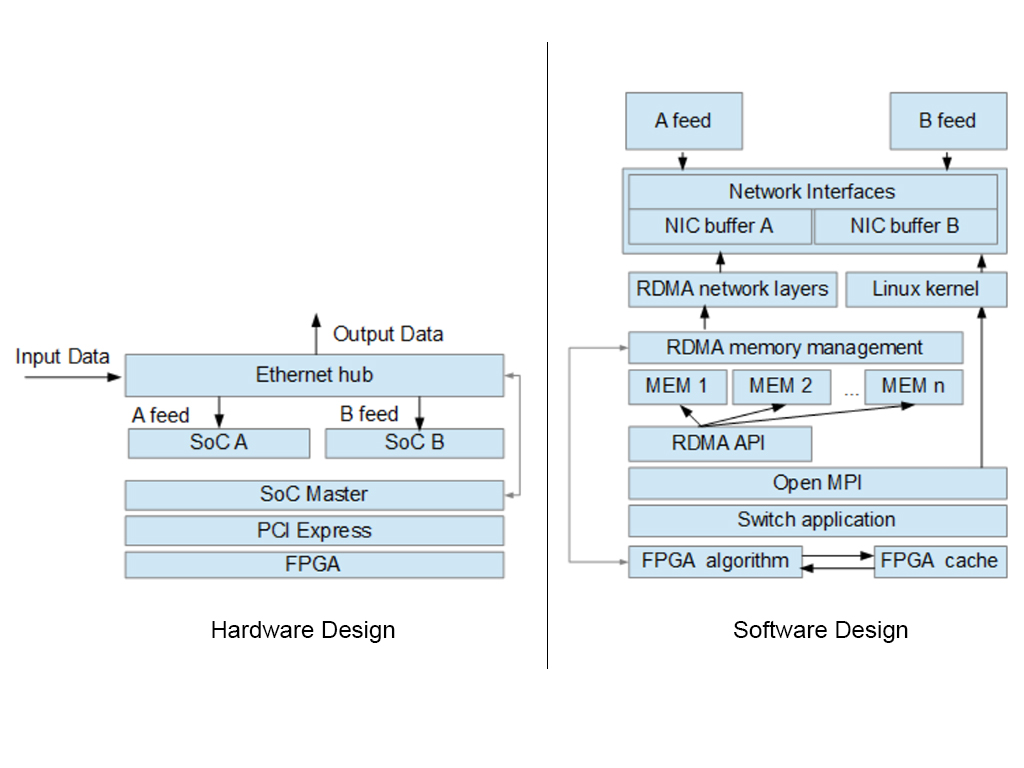
\includegraphics[width=3.5in]{picture/System_Design.jpg}
	\caption{System Design}
	\label{fig:system_design}
\end{figure}
This solution implements and improves the solution provided by the commercial firms in 10Gb Ethernet Switches, which introduces high performance computation chips to resolve the pressure in the network interface buffer. The improvement is in the layer of the high performance computing: in this solution, the HPC layer is not linked directly to the NIC in the board, but is interconnected by the Ethernet hub, which is much cheaper that 10Gb Ethernet switches. It sacrifices bandwidth in inner system to achieve similar efficiency in data processing by give spaces to heterogeneous scalable computational platforms, consisted by open sourced hardware like Raspberry Pi, and the fat-tree topology interconnection enables the cluster to expand without much cost.\\
The system can be implemented as the interconnection switch network for cloud computing clusters and high performance computer clusters. The design introduces the infrastructural solution for low-latency market data feed, utilizing data transmission efficiency with limited bandwidth, and the fat-tree topology network provides features in system monitoring and scalability in supporting massive computation.\\  
\subsection{Main Objective}
The main object for the project is to implement an experiment over a combined hardware-software environment with the features showing in table \ref{table:features}. The system is consisted of two parts:\\
\begin{itemize}
	\item The hardware part: creating physical connection among ARM based SoCs and FPGA accelerated data processor, and connect to the data feed via Ethernet cables;
	\item The software part: creating logical fat-tree topology network, that buffering dual feeds in the slave nodes and processing UDP packages via FPGA accelerated master node and other parallel user cores; 
\end{itemize}
\begin{table}[]
	\centering
	\caption{System Features}
	\label{table:features}
	\begin{tabular}{@{}l|l@{}}
		\toprule
		Features                                                                           & Description                                                                                                                                                                                                                                               \\ \midrule
		\begin{tabular}[c]{@{}l@{}}A-B data feed\\ handler\end{tabular}                    & \begin{tabular}[c]{@{}l@{}}The system needs to support dual data feed(A-B data feed)\\ to simulate the senario of ultra-low latency market data \\ transmission\end{tabular}                                                                              \\ \hline
		\begin{tabular}[c]{@{}l@{}}FPGA accelerated\\ UDP package processsing\end{tabular} & \begin{tabular}[c]{@{}l@{}}The decompression and filtering of dual UDP packages in \\ FPGA are proved to be more efficient than pure CPU \\ solutions, and can be expand to more general situations\\ in normal high frequency data networks\end{tabular} \\ \hline
		\begin{tabular}[c]{@{}l@{}}ARM based SoC \\ interconnection\end{tabular}           & \begin{tabular}[c]{@{}l@{}}Interconnection among ARM based SoC network makes it \\ possible to implement scalable buffer capacity and bandwidth\end{tabular}                                                                                              \\ \hline
		\begin{tabular}[c]{@{}l@{}}Fat tree \\ interconnect \\ network\end{tabular}        & \begin{tabular}[c]{@{}l@{}}Fat tree topology is proved to be efficient in \\ implementing interconnection network for massive parallel \\ computation, and flexible in scalable computational nodes.\end{tabular}                                         \\ \bottomrule
	\end{tabular}
\end{table}
\section{Literature review}
\subsection{Market Data Feed}
The principle of providing low latency market data feed is to provide users live data of current price information and trader status, including individual portfolio valuation, financial market data, trading activities and alarms, a matrix of these data forms an 'Order Book'. The data feeds have different price for varies delays, famous market data feed providers, or the data vendors, such as Yahoo finance, ThomsonReuters and Bloomberg provide combinations of pricing and other market information in different latencies. For example, data delayed over 5 minutes can be fetched from Yahoo finance API for free\cite{financeyahoo}, and ThomsonReuters provide paid services in different level of delay. Customers can choose to use designed data feed services to meet their business requirements, show in the reference to picture \ref{fig:1}.\\
\begin{figure}[htbp] 
\centering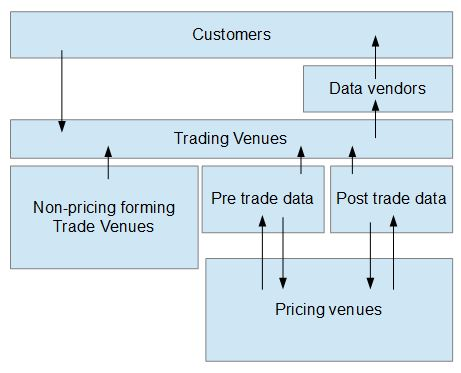
\includegraphics[width=3.5in]{picture/tradevenue.PNG} 
\caption{Relationship among trade venue, data vendors and customers}
\label{fig:1} 
\end{figure} 
\subsection{Low Latency Network Infrastructure}
Engineers provide solutions to achieve lower latency in network transmission for market data, including direct redundant fibre cables from trading centre to traders, shortest path transmission and dual data feed. For example, solution using microwave towers reducing the cost of digging tunnels for fibres and enabling signals transmit over the sphere is implemented between New Jersey and Chicago\cite{htfbackyard}, shows in the picture \ref{fig:2}. Engineers also developed 'dual-feed' mechanism to reduce the cost in retransmission when package lost\cite{zusman1999fault}.The introduction of dual feed, or the A-B feed of market data transmission uses two feeds with offset in delay to avoid significant failure such as delay or fault, especially for regional traders who want to trade across long geographical distances. \\

\begin{figure}[htbp]
\centering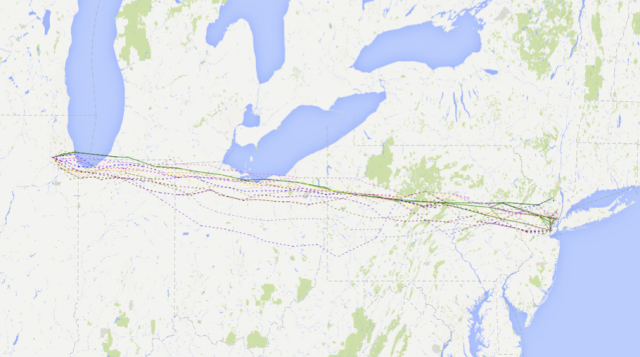
\includegraphics[width=3.5in]{picture/newyork-chicago.jpg}
\caption{Chicago-New Jersey microwave networks from data vendor Quincy Data}
\label{fig:2}
\end{figure}

\subsection{A-B Data Feed}
A-B feed structure requires two independent signals from one data provider, and the one feed(A) is several milliseconds faster than another feed(B). Relay stations between the sender and receiver need to decompress both feeds, filter and aggregate the package then transmit the data feed to the next station. Receiver also need a decompresser to handle the data from both feeds, reconstruct the original package and split the data into sub-streams forming process-specific subset of data, shows in picture \ref{fig:3}.\\
\begin{figure}[htbp]
	\centering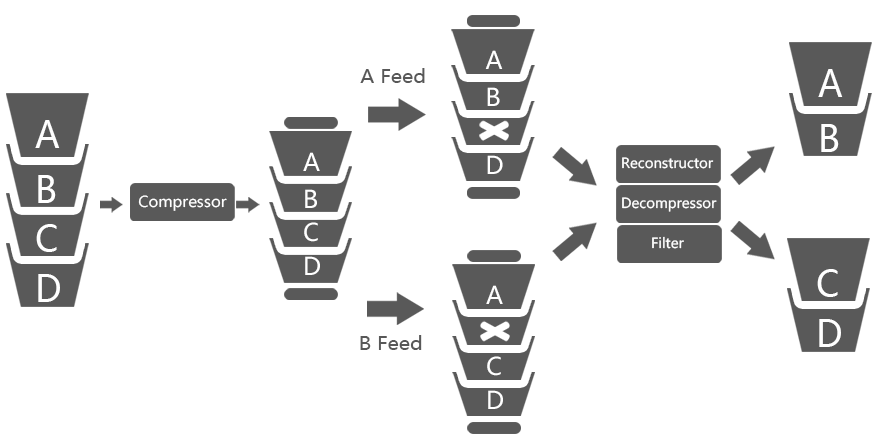
\includegraphics[width=3.5in]{picture/A-BFeed.PNG}
	\caption{Overview of A-B streaming infrastructure}
	\label{fig:3}
\end{figure}\\
Each data feed arrives in sequence with a prefixed header, containing information from abstracted layers of network protocols\cite{udpprotocol}. UDP protocol suggests UDP client to provide reliability services that the receiver should perform CRC check of the received package chains, and retransmit the chain if package lost found, timeout mechanism exacerbate the difficulty in providing low latency data service. A-B data feed reduces enable the rapid collect-dispatch system to provide output within 500 milliseconds\cite{zusman1999fault}.\\

\subsection{Scalable Interconnect Switches in Supercomputers}
Existing hardware solutions for low latency network is not suitable for mid sized institutions or individuals to start their usage of the network, and the development in building supercomputers provides an alternative solution to build infrastructure with equivalent function without implementing designed equipments.
\subsubsection{Linear Speed-up in Beowulf Architecture}
Beowulf is a highly scalable cluster architecture for computer clusters, and very popular in supercomputer design\cite{behrooz2005computer}. The basic principle is providing scalable computational power by scaling number of cores and other resources, the nodes are interconnected in proper designed network topology. The bottleneck now lies in the communication among cores in paralleled program\cite{brown2004engineering}, the bandwidth and latency in interconnect network worsen the efforts in removing the obstacles in improving the performances of the Beowulf cluster.\\
Six kinds of memory are defined according to its logical location in computer, they have distinct latency in read/write and requirements in bandwidth, shows in table \ref{table:1}.\\
\begin{table}[htb]
\begin{center}
	\caption{Latency and bandwidth in memory IO}
	\label{table:1}
	\begin{tabular}{lll}
		\hline
		& Latency              & Bandwidth Requirement \\ \hline
		L1 cache     & 1-5ns(1 clock cycle) & -                     \\
		L2 cache     & 4-10ns               & 400-1000MBps          \\
		Local memory & 40-80ns              & 100-400MBps           \\
		Local disk   & 5-15ms               & 1-80MBps              \\
		NFS disk     & 5-20ms               & 0.5-70MBps            \\
		Network      & 5-50us               & 0.5-100MBps           \\ \hline
	\end{tabular}
\end{center}
\end{table}
We set  $T_{L}$ is the total time cost for a parallel program running in a certain Beowulf cluster, and it is paralleled in n threads. Assume the ideal scenario that n is much smaller than the number of total computational cores N in the cluster, so the threads can run in separate cores without waiting. $P_{L_{i}}$ is the possibility of finding code or data in the ${i}$th type of memory, $t_{i}$ is the IO time cost for ${i}$th type of memory. We can have the expected total time cost in equation \ref{equa:1}:\\
\begin{equation}
\label{equa:1}
E(T_{L})=\sum_{i}^{n}T_{L_{i}}=\sum_{i}^{n}(\sum_{j}^{6}P_{L_{j}}t_{j})
\end{equation}
The time cost is linear related to the increment of IO times in a single core, that rapid data or code IO in one core will increase the time cost significantly.
Instructions are not loaded sequentially in L1 cache for most cases, so the bottleneck of accelerating Beowulf machines lies in reducing the swap among different memories. A simple solution is to break the memory requirements into small blocks, that the block is small enough to be swapped into L1 or L2 cache only once after execution, and runs without halt in content swapping until the result of calculation being transferred to the local memory. Master system dispatches the blocks to subsystems, and it is clear that the total time cost will be approaching to execution time of a single block when the number of subsystem increases.\\

\subsubsection{Interconnect Networks Topology: Perfect Shuffle and Fat Tree}
The Interconnect network in Beowulf clusters is important for acceleration and optimization. Performance of a supercomputer are measured by time cost in route permutations, and cost is defined by number of switching data\cite{leiserson1985fat}. For a parallel computer interconnected by boolean hypercube, the physical volume cost for a $n$ core cluster would be $n^{\frac{3}{2}}$. \\
The design of a layered interconnecting network called 'Shuffled Network' by Schwartz resolved the bottleneck in network volumes\cite{stone1971parallel}. The shuffle follows following rule, for a full set of $N$ indices, each $i$ maps into another set of indices by permutation P: \\
\begin{equation}
\label{equa:2}
P(i)=2i\; \; \; \; 0\leq i \leq \frac{N}{2}-1\\
\end{equation}
\begin{equation}
\label{equa:3}
P(i)=2i+1-N\; \; \; \frac{N}{2}\leq i \leq N-1\\
\end{equation}
and the inverse permutation 
\begin{equation}
\label{equa:4}
P^{-1}(i)=\frac{n}{2}\; \; \; (n\; is\; even)
\end{equation}
\begin{equation}
\label{equa:5}
P^{-1}(i)=\frac{n-1}{2}+\frac{N}{2}\; \; \; (else)
\end{equation}
we introduce the binary representation of data in the original set, that $i=\beta_{D}\beta_{D-1}...\beta_{1}$, so the permutation of $i$ is $P(i)=\beta_{D-1}...\beta_{1}\beta_{D}$, the inverse permutation of $i$ is $P(i)=\beta_{1}\beta_{D}\beta_{D-1}...\beta_{2}$. This defines an ideal switch network that for $o$th step, the data can be divided into even-numbered and odd-numbered processors, and in the $(o+1)$th step, data in even-numbered processors can be moved to low-numbered processors by implementing permutation $P$, and data move from odd-numbered to high-numbered processors can be performed by using inverse permutation $P^{-1}$\cite{schwartz1980ultracomputers}. The arbitrary movements of N elements in shuffle is $O(logN)$, similar to the full hypercube network while decreasing significantly in network volume\cite{clos1953study}.\\
The implementation of a perfect shuffle interconnection is the Fat-tree network. For classic parallel programs, divide and conquer is an efficient solution\cite{aho1974design}. Fat-tree interconnection strategy is a full binary tree. Message routing through children to the parent will carry data from all previous children, thus, the data capacity of the parent $cap(p)=\sum_{chil}^{route}cap(child)$.Data lost in during transmission from $child_{l_{i}}$ to $parent_{i}$ will be detected by the parent node, and retransmission will only occur between the two nodes(if the package still in the cache of the child node). The only exit is the root node, so any message route through the map will have guaranteed reliability with minimum cost.
\subsection{Field-programmable gate array(FPGA) and Integration with Open Sourced Hardware}
The introduction of Field-programmable gate array, or the FPGA, aims at solving the heterogeneous computation requirement in hardware based acceleration and general computing by using gateway logic circus to perform general algorithms or general processes\cite{hauck2010reconfigurable}. The FPGA is an integrated circuit, with re-configurable gateway and other logical blocks that can simulate most non-reconfigurable hardware with similar efficiency. The FPGA can be programmed to meet certain functional requirements by certain hardware definition languages, and modern FPGA also supports advances programming language interfaces, for example, C and Python.\\
The integration of FPGA and open sourced hardware have been carried by the community, and supported by the FPGA providers such as Xilin and Spartan. The LOGI-Pi is the very first FPGA supported by the open sourced hardware, with Spartan FX9 FPGA chip and SATA connector directly to the designed hardware board\cite{logipi}.
\subsection{Open Sourced Hardware}
Hardware engineers need to design and print their customized motherboards to support FPGA and other peripherals, however, the industry produces general motherboards supporting most of the ports including PCI-E, HDMI, USB2.0 and USB3.0. Among which the most well-known commodity hardware is Raspberry Pi and BeagleBone Black showed in picture \ref{fig:commodityhardware}. Both are designed as System On a Chip architecture.\\ 
\begin{figure}
\centering
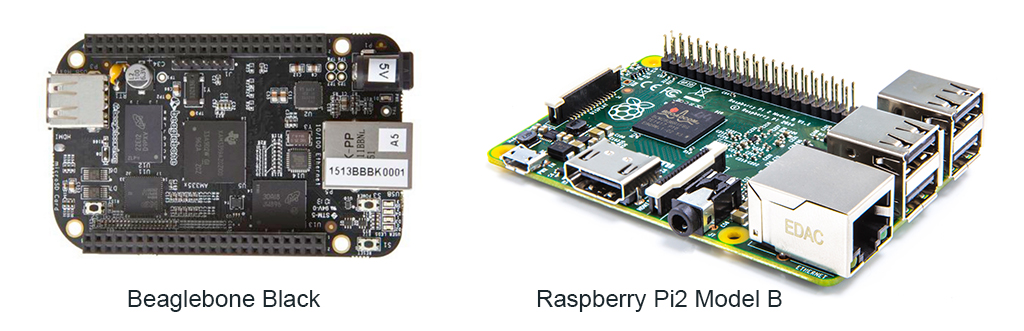
\includegraphics[width=0.7\linewidth]{picture/commodityhardware.jpg}
\caption{Beaglebone Black and Raspberry Pi2 Model B}
\label{fig:commodityhardware}
\end{figure}

\subsection{Similar Solution}
\subsubsection{FPGA accelerated market data feed}
Engineers are not satisfied with the traditional CPU based acceleration solution, and developed an alternative hardware architecture that solves the problem of buffering and filtering high frequency data. This solution introduces direct connection between FPGA chip and network interfaces, the Celoxica AMDC board enables dual feeds for single chip. Compressors and filtering program are burned in the FPGA\cite{morris2009fpga}. The acceleration of stream processing in this solution lies in the customized hardware algorithm in FPGA, and data streams goes directly to the RAM of user cores via DMA message tunnel, the IO frequency of which is higher than that in network interfaces, the structure is shown in picture \ref{fig:4}.\\
\begin{figure}[htbp]
	\centering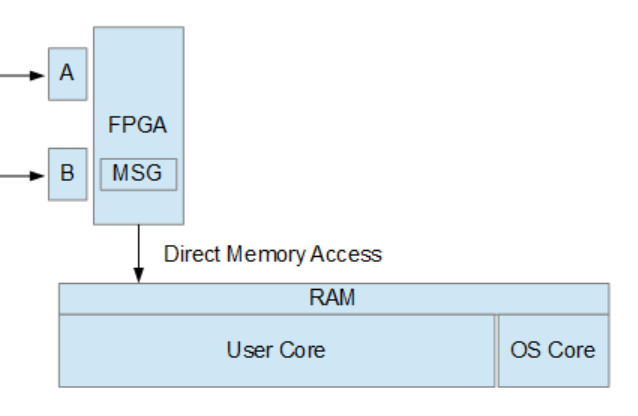
\includegraphics[width=3.5in]{picture/FPGAcall.png}
	\caption{Overview of A-B streaming infrastructure}
	\label{fig:4}
\end{figure}\\
However, this solution requires high investments in hardware, especially the motherboard and printed FPGA. Scalability is another weakness of this solution, it does not provide easy solutions for large scale implementations, especially in the scenario of bandwidth upgrading from 1Gb to 10Gb Ethernet. The NIC chip and interfaces need to be redesigned and reimplemented in the printed FPGA chip, and against the principle of System On a Chip, that the algorithm and application should be maintained only by the system supported by the hardware, not the hardware itself\cite{klaas2004system}.\\
\subsubsection{TH Express interconnection network}
TH Express interconnection network is the local area net framework for the Chinese Galaxy series super computers. It is a fat-tree topology network, and consisted of two main parts: communication network and monitor/diagnose network\cite{yang2011tianhe}. The former one connects computational nodes, the latter one checks machine status and resolves runtime error.The researchers developed a scalable network interface hardware High-Radix Routing Chip, and using RDMA method to access multiple memory spaces with unified offset, reducing processing time, improve the scalability and increasing the potential bandwidth. The architecture is shown in the picture \ref{fig:tianhe1a}\\
\begin{figure}
	\centering
	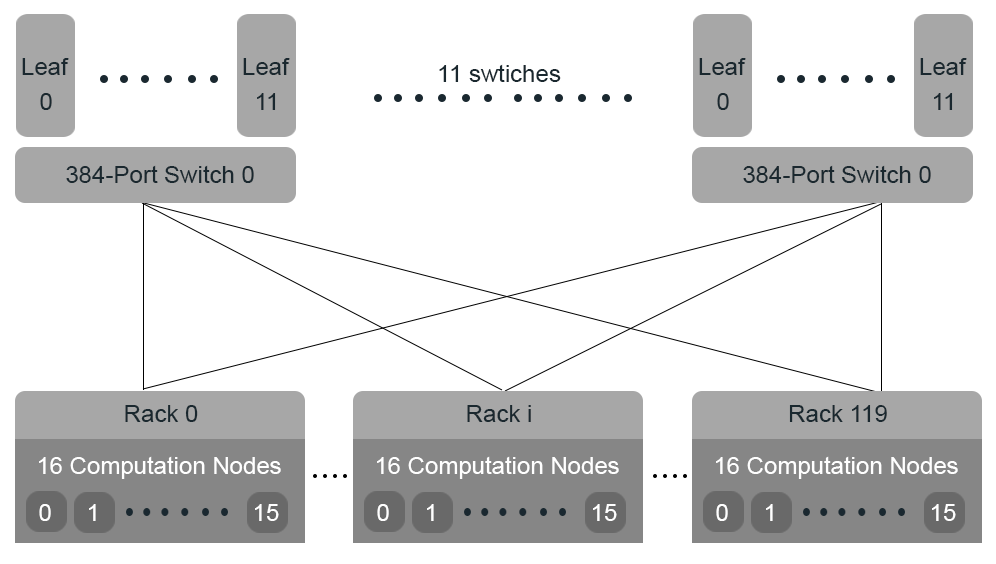
\includegraphics[width=0.7\linewidth]{picture/tianhe1A.PNG}
	\caption{Tianhe 1A interconnection network architecture}
	\label{fig:tianhe1a}
\end{figure}
Solution provided by TH Express is efficient but too expensive to achieve, however, it provides an approach to reduce latency in high frequency network data supporting the massive parallel processing system, that scalable commodity hardware supported by RDMA can improve the reliability and bandwidth of the network.\\
\subsubsection{Enyx`s ARM-based System On a Chip solution}
Market data hardware infrastructure providers offer variates of solutions to reduce the latency in market data feed. The most recent solution is to implementing FPGA hardware algorithm with ARM based SoC. It accepts A-B feed from normal network interfaces and perform the decompression and filtering via algorithm in FPGA, the ARM CPU focuses on mission dispatch and status monitor.\\
One of the well-known solution provider is the Enyx, the platform of which is based on Altera Stratix V FPGA board. The rebroadcasting latency for the FPGA supported market data processor can reach 1050 nano seconds, and average latency is 1300 nano seconds\cite{ciscoWhitePaper}. Other commercial solutions supports implementation of trading logic in the switch FPGA, that the terminals from the traders only monitors the macro status of the system, and execution of trading signals only relies on the hardware implemented applications, which reduces the event-reaction time significantly.\\ 

\chapter{Details of Implemented Technologies}
This chapter discussed the details of the four key technology in the project: Remote direct memory access, fat-tree topology network, MPI-CH, and  field-programmable gate array assisted CPU computation.\\
% Please add the following required packages to your document preamble:
% \usepackage{booktabs}
\begin{table}[H]
\centering
\caption{My caption}
\label{my-label}
\begin{tabular}{@{}l|ll@{}}
\toprule
Technology                                                               & Implementation                                                          & Details                                                                                                                                                          \\ \midrule
\begin{tabular}[c]{@{}l@{}}Remote Direct \\ Memory Access\end{tabular}   & Infiniband RMDA                                                         & \begin{tabular}[c]{@{}l@{}}Infiniband verb implementation\\ over RDMA data engine and \\ protocols\end{tabular}                                                  \\ \hline
\begin{tabular}[c]{@{}l@{}}Fat-tree topology \\ netowork\end{tabular}    & \begin{tabular}[c]{@{}l@{}}Fat-tree over\\ infiniband RDMA\end{tabular} & \begin{tabular}[c]{@{}l@{}}Fat-tree network for RDMA \\ internet layer to communicate\\ more efficiently\end{tabular}                                            \\ \hline
\begin{tabular}[c]{@{}l@{}}Message Passing\\ Interfaces\end{tabular}     & MPI-CH standard v2                                                      & \begin{tabular}[c]{@{}l@{}}Integrating the hardware platform \\ to a multi-process cluster over a \\ shared memory managed by RDMA\end{tabular}                  \\ \hline
\begin{tabular}[c]{@{}l@{}}Field Programmable\\ Gate Array\end{tabular} & Sparta FPGA                                                             & \begin{tabular}[c]{@{}l@{}}Introducing FPGA to assist CPU \\ clusters handling problems that \\ are hard to be separated into \\ paralleled threads\end{tabular} \\ \bottomrule
\end{tabular}
\end{table}
The implementation of these methods are carefully selected, to fit the architecture and achieve the best performance. MPI structure with RDMA is not a new technology, however, it has not been implemented over the dual-feed switches yet, so the design of the structure is different from a normal MPI cluster. The network topology in implementation is also another innovation because this design is usually in the computational nodes, and the project introduces fat-tree RDMA network to reduce the requirement in hardware performances of single node.\\
\section{Remote Direct Memory Access(RDMA)}
The introduction of remote direct memory access technology is inspired by the architecture design in TH Express high performance interconnection network switches, which implements the RDMA as a basic memory space management infrastructure to enable the scalability of the system using distributed cluster as an virtual switch rather than using customized central switch. The basic principle of using RDMA is to trade for efficiency with the cost of memory space and bandwidth within the switch system.\\ 
Remote direct memory access technology is developed over the traditional Direct Memory Access engine, filling the requirement of encapsulating details in data copying and shifting in cloud platforms\cite{archer2012remote}. The technology enables developers ignoring the implementation in data transmission among computation nodes, and focusing on the design of the parallel computing algorithms themselves. The actual RDMA protocol family is consisted of three protocols:
\begin{itemize}
	\item Remote Direct Memory Protocol
	\item Direct Data Placement Protocol
	\item Maker UDP Aligned
\end{itemize}
The protocol family focuses on providing data availability over the interconnected networks without operating system kernel involved, and direct data exchange in the network interfaces. The technology requires no additional buffering spaces and performs under atomic operations: read/write, send/receive\cite{RobertRDMAintro}. \\
The problem of supporting remote direct memory access is the implementation of user-level data access over traditional network protocols, which would inevitably require the interception from system kernel model\cite{liu2004high}. Remote DMA requires interception before data swapping and access in the physical memory, therefore interception in kernel model must be implemented. However, the feature required by applications that RDMA should hide the details of data shifting and other system-level details, and application structures should not be infected by the implementation. For example, data shifting within the multi-processing distribution system should not infect the processes of single threads, which may require virtual data blocks whose actual address is on the remote node. Another common scenario is the asynchronous exiting sequence of different threads, which requires asynchronous data shifting in entering and existing actual memory spaces. \\
Engineers have introduced several features in the implementation of RDMA protocols, that bypasses the kernel model in the traditional internet protocol layers, and created a virtual tunnel among buffers in the threads running on separate nodes in the cluster.\\
RDMA plays as a core part in the project, which enables the open sourced hardware performs integrated computation with incoming data feeds and share without CPU involvement,  minimizing the computational power cost by increasing the bandwidth and memory space cost, which is far easier and cheaper to achieve than high performance processors.\\
\subsection{Two Important Concepts: Verbs and Queue Pairs}
The implementation of verbs and queue pairs enables the RDMA performing kernel bypassing and CPU-free message handling. The verbs are abstract APIs that can be called in the application layer indicates that the application is implementing RDMA thus the layers below, especially the traditional socket-based internet protocol layers will be covered and the network interface card should be ready to be turned into remote memory direct access enabled model,  which will handle UDP packages with DDPP header different from other packages that it will be processed by the NIC card and sent to local memory directly with RDM protocol management. The queue pairs can be viewed as the schedule handler that performing memory registry and calling the RDMA enabled NIC, or the host channel adapter(HCA) to caring pinning of the memory packages. The basic model overview is shown in picture \ref{fig:rnic}\\
\begin{figure}[H]
	\centering
    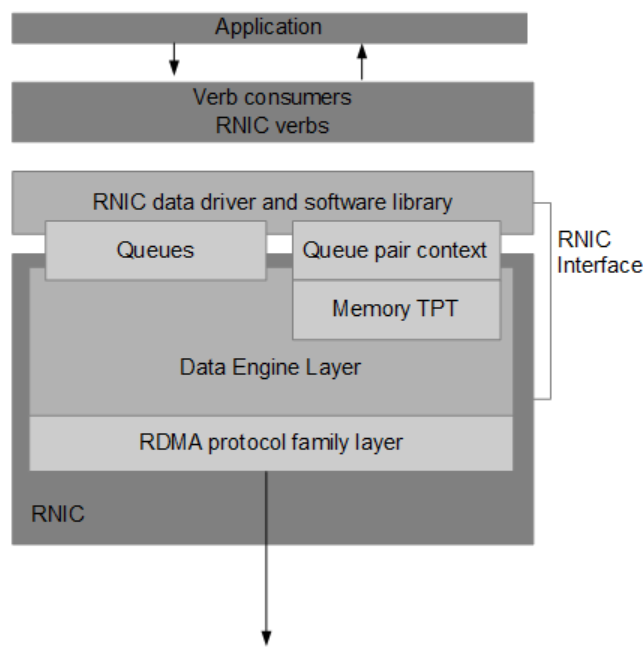
\includegraphics[width=0.4\linewidth]{picture/rnic.PNG}
    \caption{RNIC Model Overview}
    \label{fig:rnic}
\end{figure}
\subsection{Queue Pair}
The queue pair model is based on the consumer-provider model, which handling queuing of the tasks in an asynchronous way, and implements the actual data models in the network interface level to support the verb functions. The queue pair solves the problems of:
\begin{itemize}
\item Asynchronous arrival of data blocks in the interconnected network
\item Fault detection in data transmission
\end{itemize}
The queue pair is an integrated system of software, hardware and framework in remote network interface card(RNIC), and the implementation of RMDA protocol family is in the RNIC framework. The protocol family can be divided into three levels: the \(l2\) level Ethernet access mechanism implementation; the \(l3\) level IP protocol layer implementation, including IPv4, IPv6 and IPSec; the \(l4\) level protocols for TOE over TCP protocols, and RMDA protocol family including RDMA, DDP and MPA\cite{arndt2003infiniband}. RNIC infrastructure enables TCP transport support for TCP packages bypassing system kernels, which intercepts data exchange from NIC to memory. \\ 
\begin{figure}[H]
	\centering
    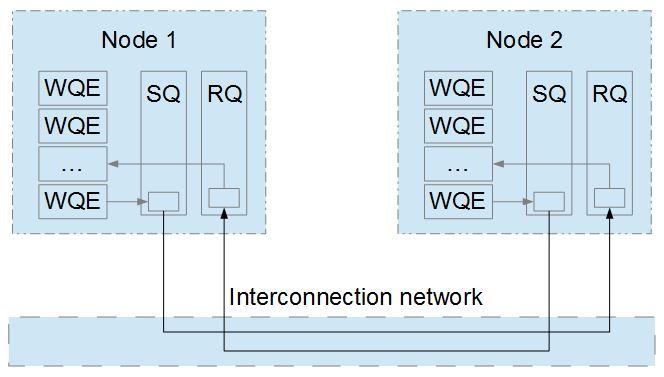
\includegraphics[width=0.6\linewidth]{picture/queuepair.JPG}
    \caption{Queued pair communication over internet}
    \label{fig:queuedpair}
\end{figure}
\subsection{RNIC Verbs}
The RNIC verbs describes the behaviour of RNIC infrastructure, and creating programming interfaces for applications to make use of the infrastructures\cite{hilland2003rdma}.  The RDMA is built upon a consumer-provider model, and the verb methods act as the middle ware between the application consumers and actual queuing pairs inside the RNIC software logics.\\ 
The verb specifications defines functions and semantics the application need to access the RDMA protocol layers, however, the verbs only include connection management and tear-down semantics, and availability to additional protocol layers  are not defined in the verbs.\\ 
\subsection{Implementation Details of Verbs}
The implementation of RNIC verbs are related to the actual policy defined by the queue pair politics, and different in actual infrastructure environment. In this project, the RDMA is the memory accessing system which provides buffering services for dynamic hardware structure for high performance system. \\
\subsubsection{Memory management}
RNIC introduces two concepts in memory management: memory window and queued pairs. The memory window manages the organization of contents in each node, and queued pairs defines the way separate nodes communicating with each other.\\
The memory windows are the basic swap element between the actual memory block and RNIC buffer\cite{garcia2006binding}. The RDMA introduces memory windows mechanism to perform memory registration and management. The remote memory shifting and offset table management are implemented through memory windows. \\
Memory space management are performed through RNIC data drivers via Tagged Offset\cite{boyd2007memory}. From the application consumer view, the memory spaces are continuous and the application can visit the entire 'shared' space by applying simple offset, but it works different from the queue pair view.\\
The queue pair is the mechanism which work requests are translated by the verbs into the interfaces provided by RNIC library, and be ready to enter the implementation of the data engine before going into the actual internet protocols. The working queues are maintained by separate nodes, and perform as the basic element of content swapping instructions. The swapping of the memory content, instructed by working queue I/O, is managed by STag access control:
\begin{lstlisting}[breaklines,breakatwhitespace,caption={STag access control},label=stag-psudoCode]
swapContentViaRNIC(QueuedProcessID qpid){
	MemoryPointer mwPointer = getLocalMemoryWindowByQPID(qpid);
	MemoryPointer mwDestiPointer = getDestiMemoryWindowByQPID(qpid);
	//Get the destination from queued pair
	ReceiveQueue rq = getReceiveQueueID(qpid);	 
	try{
		//Pop qpid from the send queue
		SendWorkingQueue.pop();				
		SwapMemory(mwPointer, mwDestiPointer);
	}catch(WorkingQueueNullException e){
		e.printStackTrace();
	}catch(MemoryException e){
		e.printStackTrace();
	}
	//Push the qpid into the receive queue
	re.push(qpid);								
}
\end{lstlisting}
So the problem lies in the strategy in choosing the strategy in the cross-node STag management. We can choose either using the same queued process id for all queued pairs, and client can seamlessly access the process registered with the same id in the server, or using different process id on each queued pairs, and managed by the client-server communication.\\
Both ways have problem: for the first solution, multiple clients can access each other`s process for they enjoy the same id in the server, which is public accessible; the second solution cannot fulfil the requirement of unified memory window management in multi-client environment, which servers need register multiple memory windows for separate clients.\\
The solution provided by RNIC is a combination of both solution:
\begin{itemize}
	\item At binding phase: queued pair id binds with each memory window, and different in separate nodes;
    \item At accessing phase: memory window with QPID is registered in both source and destination paired queues with same QPID;
\end{itemize}
\section{Fat-tree topology implementation over RDMA}
\subsection{Reducing the Cost in Node Intercommunication}
Cost in node intercommunication lies in to aspects: the content transmission speed between the network interfaces and memory spaces, and the latency in data links among nodes.\\
Data swapping within RDMA system is a bandwidth consuming performance, and the efficiency in data transformation is the threshold for the overall efficiency of the system. \\
In the data engine level, NIC can access the data blocks with the direct memory addresses without CPU, and improving the accessing speed of data by direct I/O performances from NIC to memory. 
\begin{lstlisting}[breaklines,breakatwhitespace,caption={Direct Data access from NIC to memory},label=nic-psudoCode]
SwapMemory(Memorypointer source, Memorypointer destination){
	//The pid in different client is different
	QueuedProcessID destiPID = receiveQueue.pop().getPID;
	Memorypointer desti = 
		destination + getOffset(source, destination);
	try{
		kernel.directWriteToMemory(desti,destiPID.getContent());
	}catch(MemoryIOException e){
		e.printStackTrace();
	}  
}
\end{lstlisting}
In the network topology level, the RDMA network protocols introduces fat-tree topology, which 'parent' nodes have the bandwidth aggregating bandwidth of all children nodes, and the perfect shifting mechanism guarantees the minimum cost in data shifting.\\
The implementation of perfect shifting is based on one assumption: most of instructions performed by applications require data from adjacent memory blocks $T_{i+1}(d)=Addr_{i}+V(T_{i}(d))$, therefore, the 'next step' data requirement process always requiring data either:
\begin{itemize}
	\item Require data from local memory space
    \item Require data from the neighbour nodes with the same parents
\end{itemize}
The implementation of dual feeds in data sources also reduces the time cost significantly, for the bypassing of kernel model in UDP package processing, the client in the network interface in switches works different in error processing, and node level error can be detected in leaf level switch. Comparing to flat structured centralized switch, the fat-tree topology interconnection reduces the expected error detection time from $E(T_{t}|e)=E(T_{node}|e)+E(T_{route})$, however, the expected time of processing error in node($T_(node)$) is a constant, assuming the cluster is homogeneous, and reducing the error processing time in network transmission phase.\\
\subsection{Analysing flat topology and fat-tree topology}
\begin{figure}[H]
	\centering
    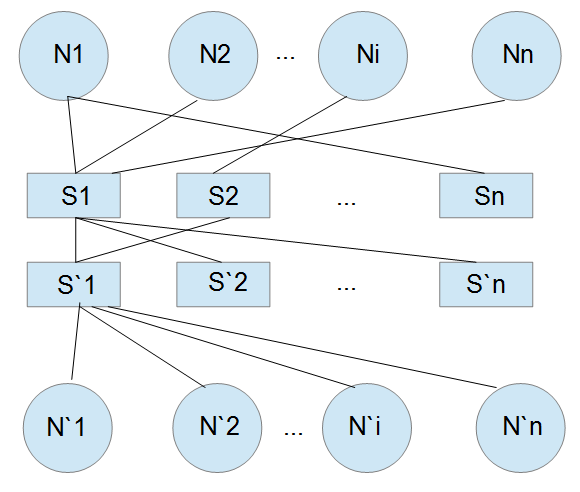
\includegraphics[width=0.4\linewidth]{picture/FlatStruct.PNG}
    \caption{Flat structured network}
    \label{fig:flat}
\end{figure}
The nodes can be divided into three groups according to the topology position to each other:
\begin{itemize}
	\item Adjacent nodes: nodes have the same parent hub
    \item Non-adjacent nodes in the same field: nodes have different parent hubs, but the hubs have direct interconnection
    \item Non-adjacent nodes in different field: nodes have different parent hubs, and the hubs have no direct interconnection
\end{itemize}
As shown in picture \ref{fig:flat}, the $N_{i}$nodes can detect and process errors in transmission and calculation, and $S_{j}$ works as the network hub which cannot process data errors. The average processing time from node N1 to adjacent nodes in network can be divided into three parts:\\
% Please add the following required packages to your document preamble:
% \usepackage{booktabs}
\begin{table}[H]
\centering
\caption{Average processing time for node N1}
\label{tab:n1proc}
\begin{tabular}{@{}ll@{}}
\toprule
Equation                                                                                          & Comment                                       \\ \midrule
$E(T_{adj})=T_{\widehat{N_{1}S_{1}N_{i}}}=\frac{\sum_{1}^{n}T_{i}}{n}$                            & i is the adjacent node                        \\
$E(T_{\widehat{N_{1}S_{1}{S}'_{1}N_{j}}})=2\times E(T_{adj})+2\times T_{\widehat{S_{1}{S}'_{i}}}$ & j is the non-adjacent node in different field  \\
$E(T_{\widehat{N_{1}S{N}'_{k}}})=2\times E(T_{adj})+E(T_{\widehat{S_{1}{S}'_{i}}})$          & k is the non-adjacent node in the same field \\ \bottomrule
\end{tabular}
\end{table}
From the equations it is easy to observe that the most time-consume process is the error detection when data is route through different fields, however, this could be frequent even we assume that the instructions in most cases process data in the adjacent node, because the switch nodes in different nodes in the node cluster, for example, $N_{1}$ and ${N}'_{1}$ could be logically adjacent in the computational cluster it connects to.\\
There are two options to reduce data processing time in the switch cluster shown in the table \ref{tab:n1proc}, one is to make all nodes adjacent to each other, however, the structure of the centralized hub could be over-complicated, another one is to to connect all the fields together,the problem is the complexity in constructing the interconnection network. A full mapping among the field hubs requires each hub supporting bandwidth of $bandwidth_{n}\times n_{fields}$, which can be very costing if we need to implement the high bandwidth in each field node.\\
One possible solution to avoid the increment of bandwidth requirement is to implement layered interconnection network rather than a flat structure, which resolve the bandwidth requirement to the back bone layer rather than the entire communication network. \\
\begin{figure}[H]
	\centering
    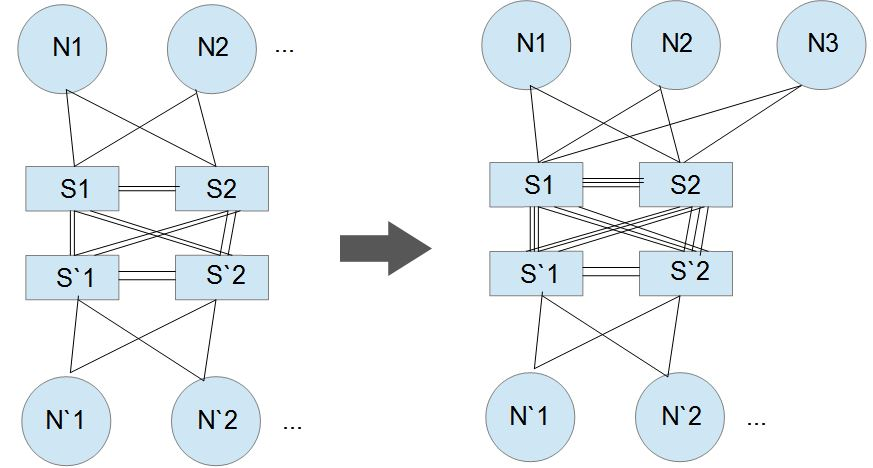
\includegraphics[width=0.5\linewidth]{picture/flat_addNode.JPG}
    \caption{Adding one node in flat mapping in the same field, six connections are changed}
    \label{fig:flatadd}
\end{figure}
The implementation of a tree-structure properly solves the problem, which not only provides a layered infrastructure which implements an aggregating bandwidth requirement from leaves to the root upstream, but also ensures the scalability of the system at the minimum cost, and the binary tree search time is $log(N)$ \cite{ellis1980concurrent}, because the increment in leaves only affects the sub-nodes in certain fields, rather than the entire system.\\
\begin{figure}[H]
	\centering
    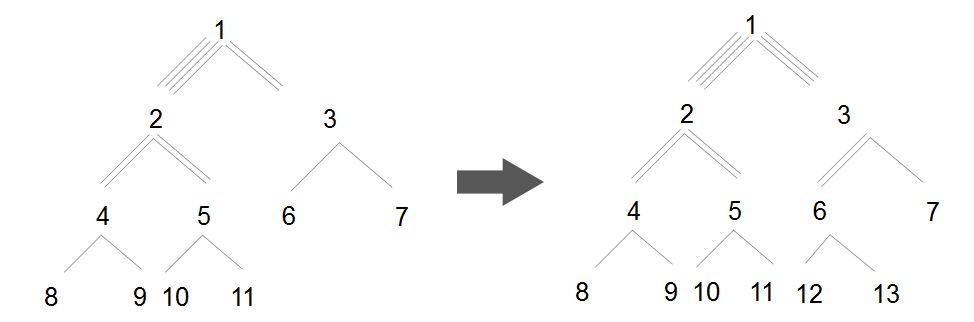
\includegraphics[width=0.6\linewidth]{picture/tree_addNodes.jpg}
    \caption{Adding nodes in tree structure, only two interconnections are changed}
    \label{fig:addnode}
\end{figure}
\subsection{Rebalancing the fat-tree over network bandwidth}
Another benefit of introducing the tree topology is the quick rebalancing feature of a tree topology network. The unbalanced tree will cause an unbalanced bandwidth load in the system. Advanced algorithm can rebalance the tree from a vine to a balanced binary tree with the time complexity of$O(n)$, and the amount of the nodes only have linear affect on the rebalancing practises. The extreme situation is a $m$ depth vine, whose root only have one leaf in one side, and another vine with $m-1$ depth vine.\\  
First, introducing the compressing of a vine in the rebalancing:
\begin{lstlisting}[breaklines,breakatwhitespace,caption={Direct Data access from NIC to memory},label=compression-psudoCode]
compression(NodePtr root, Integer count){
	NodePtr scanner;
	NodePtr child;
	Integer i;
	scanner = root;
	for i from 1 to count{
		child = scanner.right;
		scanner.right = child.right;
		child.right = scanner.left;
		scanner.left = child;
    }
}
\end{lstlisting}
and the steps from $k$th compression to $(k+1)$th compression can be shown as the figure below:
\begin{figure}[H]
	\centering
    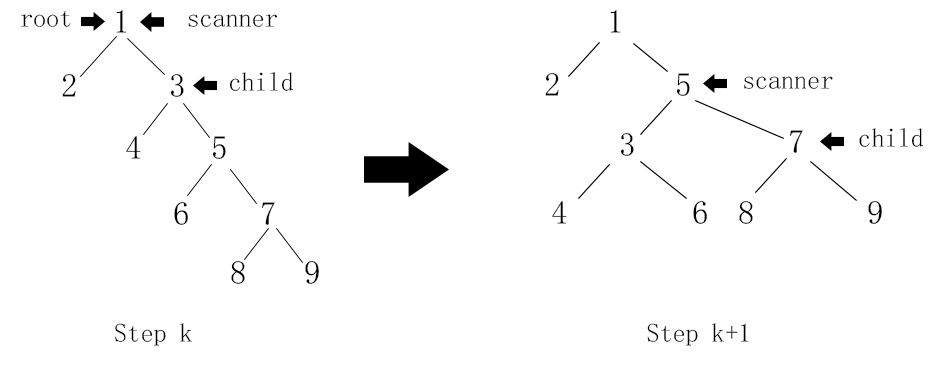
\includegraphics[width=0.6\linewidth]{picture/compression.JPG}
    \caption{Compression step k to step k+1}
    \label{fig:compression}
\end{figure}
The compression process will be performed each turn in rebalancing, for an vine with $n$ depth, each step will make a compression of the rest $\frac{n}{2}$ branches, and the node of the vine can be a complete binary tree, take the example showed in picture \ref{fig:compression}, nodes 2,4,6,8,9 are all complete binary trees, and the compression will not change the structure of the binary threes, because the only the vine nodes 1,3,5,7 are changed by the compression process\cite{stout1986tree}.\\
The rebalancing of the tree structure resolves the balancing problem of interconnection bandwidth, take the bandwidth requirement of node 5 for example: in step k before rebalancing, the bandwidth requirement of node 5 on the left side is $b_{1}$ for only one node, and on the right side is $\sum_{m}b_{i}+1$, $m$ is the amount of the leaves after vine node 5. After rebalancing, the bandwidth of node 5 on each side is the same($2\times B_{b}$, $B_{b}$ is the bandwidth of a balanced tree).\\ 
The introduction of rebalancing tree in the network topology of fat tree is for the stable scalability, and new nodes adding to the system will not have to be added following certain topology rules: the balancing of bandwidth requirement are maintained by the master node automatically, and the topology of the system is maintained dynamically.\\
\section{RDMA verb implementation: Infiniband Verbs}
Infiniband verbs, or the iverbs, are the verbs supported by infiniband RDMA protocol family which supports the implementation of RDMA over general hardware clusters. The build-in network topology management can be configured into fat-tree, which is discussed above that we want to introduce in the system. \\
The Infiniband provides upper-layer protocols(ULPs) supporting not only RDMA itself, but also most features in MPIs. The reason not using the entire Infiniband protocol family is that the support of message passing interfaces in infiniband is ill-supported in scalability, and the version we use for multi-processor interface for the open-source hardware cannot perform ideally in the infiniband pre-configuration, because the passing interfaces designed in the iverb is for much heavier use, including distributed service providers and computation. Our system is a pure message passing system which only filtering and passing message for the clusters, rather than perform the computation for them.\\
The iverb implementation can be divided into two parts\cite{bedeir2010building}. The client part and the server part. Server side mainly listens to the sockets, and react to the sockets send from the client side. The client send sockets to the servers in order to fetch data from memory directly via RDMA mechanism.\\ 
The iverbs lie in the client side when the application need to communicate with the server(the details are hidden by the verbs) to fetch data and instructions, and the server side when request are queued in the memory spaces, verbs will translate the queues to working queue elements and find the memory windows it points to, reply with the correct memory space addresses to the client to fetch the data.\\
Two features must be guaranteed for the full functioning of iverb system:
\begin{itemize}
	\item Asynchronous reliable communication: both sides will receive hanging notifications and instructions 
    \item No buffers in application level: the synchronization of the send-receive system requires no buffering especially in application memory spaces, which will cause serious problems if the content of application data is modified after sending without completing.
\end{itemize}
\subsection{Building the Passive Side}
The passive side creates and maintains an event handler for queue pairs and an event listener running in the background of network interfaces, which listens to the events from the active sides and send request queues to the queue pairs in the queue event handler directly without implementation of CPU. The iverbs in the event handler will then send the response including the memory content to lower-level protocols to be packaged into sockets, and the network interfaces will then send the package to the destinations.\\
\begin{figure}[H]
	\centering
    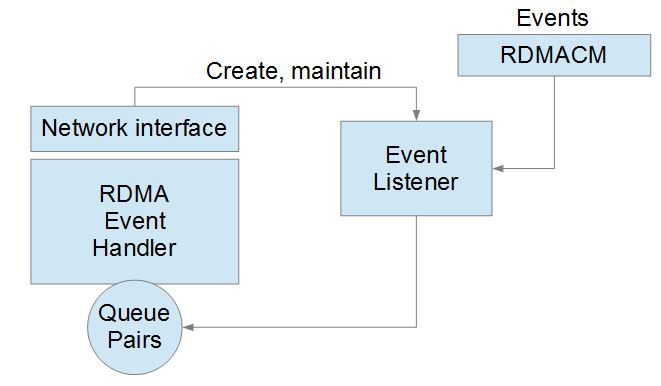
\includegraphics[width=0.6\linewidth]{picture/passive.JPG}
    \caption{Passive side design}
    \label{fig:passive}
\end{figure}
\subsubsection{Building the Active Side}
The active side runs in the client, which directly queries the content from the 'virtual' memory spaces, which is managed by the server. The active side runs a queued event handler which consumes working queue elements translated by the iverbs from the applications, and resolves receiving queues from the server, getting the actual content of the shared memory spaces.\\
The active side maintains a route to peer nodes for both active and passive sides, in order to communicate among the clusters for swapping data and instructions.\\
\begin{figure}
	\centering
    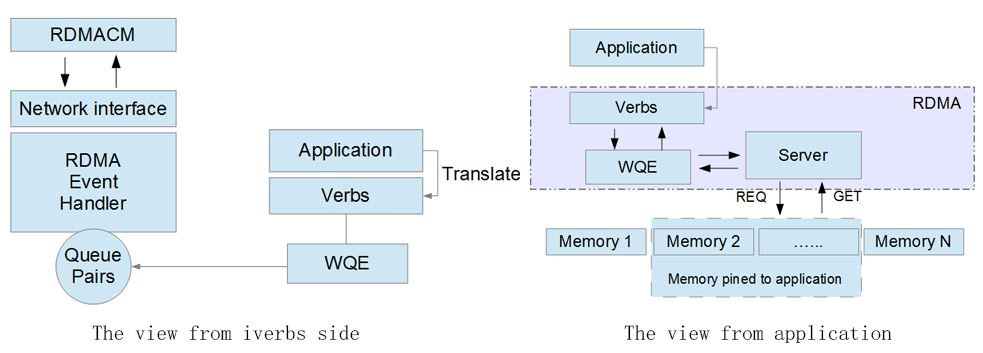
\includegraphics[width=0.8\linewidth]{picture/active.JPG}
    \caption{Active side design}
    \label{fig:active}
\end{figure}
\subsection{Conclusion}
This section introduces the RDMA method for memory management, and the fat-tree topology we need to implemented assisting the RDMA for better performances.\\
The purpose of implementing RDMA in the project is to overcome the weakness in computational power in open-source hardware, which is usually based on ARM processors with limited memory spaces. The established commercial solution to this problem usually contains an unified memory flash.The RDMA enables us to introduce fragmented memory hardware into an virtually unified one. \\
The purpose of implementing fat-tree topology is inspired by the TH-Express high performance computation clusters, which uses fat-tree interconnection network to solve the problem of low-latency network infrastructure\cite{pang2014th}. In this particular project, fragmented nodes makes it different than implementing a centralized routing system, which have fixed bandwidth balance. The implementation of rebalancing load among node clusters makes it possible to dynamically add/remove nodes.\\
\section{MPI-CH}
Researchers introduce the MPI to build a portable and scalable multi-threading platform over heterogeneous hardware environment\cite{dongarra1995introduction}.To understand the necessity of this interface, a brief introduction of message passing model need to be introduced.\\
Most parallel applications were for scientific purposes\cite{kendall_2016}. Most of the libraries for such applications uses a message passing model for exchanging data among different cores of the machine, and normally a master manages multiple slaves by dispatching tasks and gather results.\\
The MPI-CH is an implementation of the message passing interface standard, and is widely used over multi-processing machines as a data exchange model over multiple processors performing multi-threading computations. It covers almost every aspect of MPI standards, and widely supports far more different hardware architectures compared to another well-known implementation, the OpenMPI.\\
The MPI-CH is the solution for implementing scalable dual-feed receiver in this project, to enhance the efficiency of communication among the nodes using a message passing interface, instead of building a complicate interconnection structure from ground zero. The project makes use of the listing features from MPI-CH compare to other solutions:
\begin{itemize}
	\item Easy to build and configure message passing interfaces
	\item Remote memory access mechanism to enable the scalability
	\item Fat-tree topology to balance the efficiency in hardware architecture of single nodes and network bandwidth
\end{itemize} 
\subsection{Introduction to SPMD and MPMD}
A parallel application can be divided into two different kinds according to the way it uses data and instructions, Single Program Multiple Data and Multiple Program Multiple Data.\\
Before introducing the SPMD and MPMD,it is necessary to make a brief introduction to the concept of Single Instruction Multiple Data(SIMD) and Multiple Instruction Multiple Data(MIMD).\\
SIMD is the model that each node execute same machine instructions over different data, for example, for array ${A}$, executing $A_{i}+1$ on each element of ${A}$ can be performed by a SIMD process by implementing the ${plus 1}$ method on each paralleled cores. MIMD works in a different way: for calculation of equation $A+B+C-D+E\times F$ , an MIMD implementation can divide the calculation into $(A+B)_{node1}+(C-D)_{node2}+(E\times F)_{node3}$ to three nodes with different instructions.
Both SPMD and MPMD are the subsets of MIMD\cite{darema2001spmd}. In this project, MPI-CH library supports both SPMD and MPMD mode, the system can differ the model by using the command line tool indicating how the program and data being seprated.\\
\subsubsection{Single Program Multiple Data}
Single Program Multiple Data(SPMD) is the parallel application which only implements one application, and execute it among each node with different sets of data.\\
A good example of message passing model is a shellsort process: for an $l$ length array $A_{l}$, the shellsort process divides the array into $\frac{l}{mod(\frac{l}{2})}$ fragments, and perform quicksort process on each fragment.The quick way to improve the efficiency of the algorithm is to place each quicksort process on a independent computational core, therefore, the time complexity only depends on the strategy of choosing the length of steps $mod(\frac{l}{2})$. However, it leaves a problem of communication among the cores.\\
For step $k$, the algorithm uses $n$ amount of cores, and in step $k+1$, the content in the memory space of each core will have the following two steps:
\begin{itemize}
	\item{1.} Merging together into a new array ${A}'$
    \item{2.} Dividing ${A}'$ into $\frac{n}{2}$ fragments and dispatching them to $\frac{n}{2}$ cores
\end{itemize}
Therefore, the programmer only need to design the dispatching mechanism and quicksort algorithm in each core. However, the solution could be cumbersome to achieve without MPI model due to the fact that for each step, the number of cores need to wake and perform send/receive practises will be different, and the designer need to predict the number of cores in each step. However, the time cost in communication is very high as the centralized node need to communicate to each node two times each step.\\
\subsubsection{Multiple Program Multiple Data}
Multiple Program Multiple Data performs parallel practises in a different way. Take the shellsort for example, if the parallel application is running on a heterogeneous cluster, whose node has different software and hardware structure and the programmer need to design and implement different sorting algorithm on each node. Therefore the step $k$ to $k+1$ could be:
\begin{itemize}
	\item{1.} Merging the fragments into new array ${A}'$
    \item{2.} Querying the infrastructure library and forming the dispatching strategy for step $k+1$, including the number of nodes, structure of the implemented nodes and data requirements for each node
    \item{3.} Implementing $k+1$ step, and divide the array ${A}'$ into required fragments, transmit the data into the destination
\end{itemize}
The MPMD program is hard to design due to the difficulty in managing the data fragmentation process, which differs according to the configuration of each node.\\
MPI-CH implements both SPMD and MPMD models, and the host can differs the structure by using command line to submit tasks from master to slave nodes.
\subsection{The architecture of MPI-CH}
The core part of MPI implementation is the send-receive pair between processes, forming a programming interface following certain message protocols with semantic specifications over varieties of machine implementations.\\
The architecture of MPI-CH standard can be abstracted as the picture below:
\begin{figure}[H]
\centering
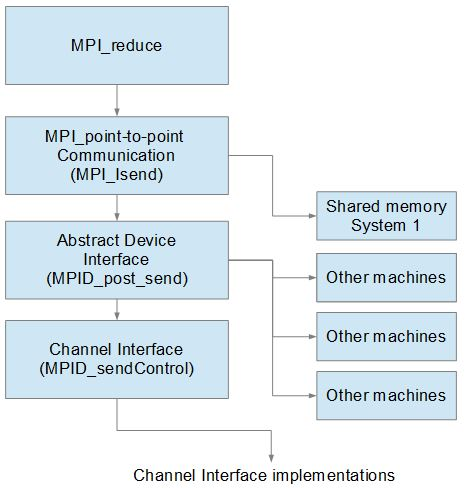
\includegraphics[width=0.6\linewidth]{picture/MPIarchitecture}
\caption{MPI architecture}
\label{fig:MPIarchitecture}
\end{figure}
The design for the MPI-CH infrastructure follows the following principles\cite{gropp1996high}:
\begin{itemize}
	\item Sharing code without compromising in performance over the actual implementation
	\item The MPI-CH should be easy to dock on different platforms with minimized amount of code changing
\end{itemize}
The first principle is to meet the need of re-implementation lower-level objects in MPI implementations over opaque objects, including communicators with tags on it, because most of these contents in MPI-CH is platform independent, and code sharing will solve the problem of dynamic scalability. The second principle requires modularised design of the infrastructure, which can replace the platform independent modules, especially the sharing part, easily and dock to the platform with minimum cost.\\
The implementation of MPICH can be split into three levels according to the sequence from application to the actual hardware.\\
\subsubsection{MPI API}
The MPI reduce, or the MPI API for the applications, are the highest layer which implements user-level abstract objects and the user applications can introduce these elements to get access to MPI-CH managed resouces.\\
The high portability feature of MPI-CH makes the interfaces easy to use and independent to actual hardware. One application can run on different MPI-CH supported hardware clusters by using configuration parameters. The entire application can be wrapped by two functions: MPI\_Init(num\_arg,*vec\_args) and MPI\_Finalize(). The program can perform both SPMD and MPMD inside the curve, and the MPI standard does not define the behaviour inside body\cite{mpich_doc}.\\  
\begin{lstlisting}[breaklines,breakatwhitespace,caption={Example of using MPICH initialization-finalization pair in C},label=compression-psudoCode]
#include<mpi.h>
int main(int argc, char** argv){
	MPI_Init(NULL, NULL);
	int processor_size;
	MPI_Comm_Size(MPI_COMM_WORLD, processor_size);
	int processor_rank;
	MPI_Comm_Rank(MPI_COMM_RANK, processor_rank);
	char processor_name[MPI_MAX_PROCESSOR_NAME];
	int name_len;
	MPI_Get_processor_name(processor_name, &name_len);
	/*-----------------/
	/ Perform algoritm /
	/-----------------*/
	 MPI_Finalize();
}
\end{lstlisting}
\subsubsection{Communication mode in MPI}
It is essential to introduce the communication mode defined in the MPI standard before moving to the actual implementation. The MPI standard defines four communication mode: \textit{Standard}, \textit{Synchronous}, \textit{Buffered} and \textit{Ready} modes\cite{dimitrov1999efficient}. It is easy to understand that RDMA always need to transfer small amount of data in high frequency over the network, therefore the protocol strategy cannot be too complex. The RDMA introduces rendezvous communication protocol to perform the transmission.\\
\begin{figure}[H]
\centering
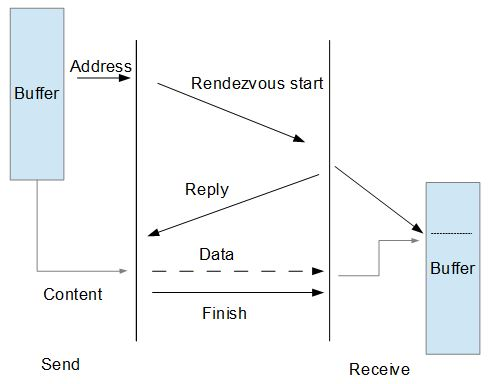
\includegraphics[width=0.6\linewidth]{picture/rendezvousMode}
\caption{Rendezvous communication in RDMA}
\label{fig:rendezvousMode}
\end{figure}
This zero-copy rendezvous protocol in RDMA works in the following sequence:
\begin{itemize}
	\item[1.] The buffer address is wrapped into control messages and transmitted to the receiver
	\item[2.] The receiver decodes control message and find the address in the receiver`s buffer, and send acknowledge message to the sender
	\item[3.] The sender sends data to receiver, and send finish segment when the transmission is finished
\end{itemize}
It uses eager strategy in pushing data to the receiver, however, there are still problems in this send-receiver strategy, especially when MPI implements the RDMA feature. The problem will be discussed afterwards.
\subsubsection{Abstract Device Interface}
The MPI-CH implements the mechanism Abstract Device Interface(ADI) in order to provide abstract services for the upper level functions, and hide the details of hardware implementations to the applications\cite{gropp1994abstract}. The message passing happens in this layer when the application uses MPI\_send or MPI\_receive, which indexed by the \textit{handle}, and queued in a way to ensure the execution sequence. The queue is managed by the MPI-CH directly and abstracted from the hardware implementation, and the handlers of IO behaviours are invoked by the lower layer, which slurp the contents and package them into proper format to suit the requirement of different mediums. The descriptions in handlers defines the type of interfaces it needs to be invoked.\\
The idea for the ADI design is to abstract the communications among nodes, and parallel scheduled from the view of applications should have no difference between local cores and remote ones. This due to the fact that MPI standard defines only the local performances in the first version of standard, and the development in network technology enables the hardware designer to introduce remote resources into a bundled parallel computing structure\cite{liu2004high}. 
ADI contains three queues: \textit{send\_queue}, \textit{posted\_recv} and \textit{unexpected\_recv}.
Send queue is for the outgoing messages, and the other two are for receiving messages. The reason for dual queues for receiving is for the asynchronous communication. Application can have the two scenarios when receiving the message from other nodes in MPICH:
\begin{itemize}
	\item The application is ready for receiving a message, and send \textit{MPI\_recv} request to the ADI layer via the API
	\item The application is not ready for any new messages, however the ADI layer receives a message with the handler pointing at this node
\end{itemize}
The first one will trigger an content shift from the queue manager to the application buffer with required contents in the queue, and the second one will register a description in the MPICH runtime manager, which enables that when the application calls for the content from receiving queue it can be shifted to the user buffer directly. \\
Another queue the ADI manages is the device ranking queue, and this queue is initialized by the user when the distributed application is deployed. It contains all the devices the MPICH runtime manager have access to, and abstract the invoker as an communication interface. The application do not need to know the existence of this list, and by invoking the communication interface, runtime manager will post the messages according to the pre-configured ranking list after an outgoing handler is created. When receiving the queue, runtime system will fairly threat all the resources, and no priority in receiving queues. The ADI uses an round-robin style of circulating query around the devices and asks if there is a new message\cite{protopopov2001multithreaded}.\\

\subsubsection{RDMA channel implementated on ADI3}
MPICH introduces ADI3, the Abstract Device Interface version three, which enables programmers to implement their own communication strategy among nodes. The structure of ADI is consisted of two parts, and can be presented in the following fashion:
\begin{figure}[H]
\centering
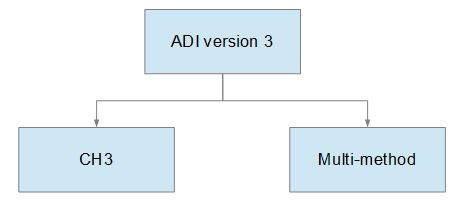
\includegraphics[width=0.5\linewidth]{picture/ADI3}
\caption{Structure of ADI3}
\label{fig:ADI3}
\end{figure}
The CH3 is a bundle of functions which implements the interfaces for different format of communications, including TCP socket and SHEMEM channel. The reason to abstract these interfaces in a subclass of ADI3 is that the CH3 bundles them into \textit{channels}\cite{mpich_doc_adi3}. The channels are based on normal Unix based socket, and introduces features such as queuing and listeners to achieve better performances.\\
The implementation of RDMA over MPI-CH structure is introduced via this mechanism, because the ADI is consisted of a set of macros and functions which allows varieties of different software-hardware infrastructure to be implemented. The design of this mechanism allows the connected hardware to implement their own message queues and data processors, which is required by the RDMA verb mechanism which overrides the kernel model in UDP socket processing and memory management by introducing its own network data exchange protocols. The RDMA channel only contains five functions, and will be discussed in the next subsection.\\
\subsubsection{RDMA channel implementation}
RDMA channel is designed for global memory share mechanism. It contains two functions for communication, \textit{put} and \textit{get}. Other three functions are for process management. Shown in the discussion of RDMA above, it maintains a queue between two nodes separately.\\
Both \textit{get} and \textit{put} are non-blocking, and the data they manipulate can go directly into the queue rather than wait until the entire process to finish. It is easy to see that the actual implementation of these two functions are different from RDMA standard description, whose communication methods are one-sided, but the actual implementation in CH3 is two-sided.\\
\begin{figure}[H]
	\centering
	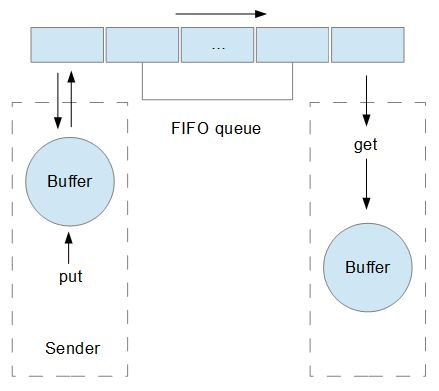
\includegraphics[width=0.5\linewidth]{picture/senderreceiver}
	\caption{The message queue between nodes}
	\label{fig:senderreceiver}
\end{figure}
The put-get pair can manipulate the buffer in a straightforward fashion, and the memory buffer can be viewed as an circle: the pair holds an fixed size buffer with an fixed head index, and the put method can insert contents into the circle start from the head buffer, meanwhile the get method invoked by the receiver can read contents also start from the head index and points at the tail. Therefore, the buffer\_read method, which is time consuming, can be asynchronous with the buffer\_write, as long as the buffer is not full. This way of communication also makes it easy to synchronize the memory addresses between the sender and receiver, because the communication buffer uses only one header index and both put and get starts from the same place, only with the opposite direction in the circle.\\
The reason of implementing an independent RDMA channel over CH3 rather than creating a new subset of communication protocols of ADI3 is:
\begin{itemize}
	\item Modern implementations already have similar shared memory mechanism in CH3 layer, and the improvements in a subset of CH3 can inherit the interfaces of CH3 itself, and other system built purely on CH3 can benefit from it
	\item Potentially, other MPI mechanisms will be introduced into the MPICH implementation, for example the Infiniband RDMA which discussed above that it has one-side communication method, and the new implemented methods can use the RDMA channels by following the CH3 interfaces
	\item The portability requirement of MPICH design makes it necessary to consider a general design of communication channel rather than a specific one
\end{itemize} 
\subsubsection{The fat-tree topology}
In this project, the RDMA channel performs as an optimized data exchange channel for the received data, however, the CH3 does not define the way RDMA channel organizes the network topology.\\
As discussed in the RDMA section, the best practise for RDMA performance is to implement fat-tree topology within the cluster, especially under the circumstance that nodes are not powerful enough to process complex computation tasks, therefore the design of software implementation over the cluster needs to sacrifice the bandwidth resources to achieve better overall performance with ARM based CPUs.\\
The fat-tree topology pairs the dual-feed receivers as leaves of the bottom layer, along with an upper layer node also supported by ARM CPU, the added bandwidth among the three nodes is equal to the output.
\begin{figure}[H]
\centering
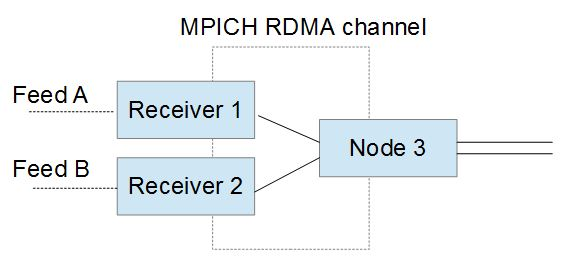
\includegraphics[width=0.7\linewidth]{picture/fattreeimpl}
\caption{Fat tree implementation}
\label{fig:fattreeimpl}
\end{figure}
We expect the RDMA in MPICH can reduce the requirements computational power of each receiver, and the parent node $node_{3}$ can have better hardware support to perform more complex algorithms compared to the receivers.\\
\subsection{Conclusion}
This section explains the logical structure of the system to implement the dual-feed receivers. Using the MPI-CH implementation under two parallel Raspberry Pi hosted applications, the system can achieve the goal of receiving dual feeds without implement expensive hardware which solves the problem by implementing parallel hardware bus between the CPU and two or more NIC cards. This section also explains how the three important parts works in the background: message queues, remote memory access implementation and fat-tree network topology. The next section will talk about how the third Raspberry Pi works as the master node connecting to a FPGA.\\
\section{Field Programmable Field Array(FPGA) Assisted Computation}
This section introduces the advanced hardware implementation on the $node_{3}$ discussed above. The Field Programmable Gate Array, FPGA is transitionally considered independent from the general computation architecture such as the CPUs, however, recent development in hardware pipeline technology enables the FPGA to communicate with the general architecture directly, and the content swap from FPGA to CPUs are much faster than the network supported data transmission.\\
FPGA is known for handling single threaded tasks which are hard to be split into sub-tasks, or the resources for parallel computing is much more costing than those for the single threading processes. FPGA is performs all the computation tasks via hardware directly, and they are programmable.\\
The project implements FPGA to support the \textit{merging} process after the cluster receiving the data feed. Discussion below shows the details of following technologies:
\begin{itemize}
	\item Sparta-6 integration with Raspberry Pi
	\item FPGA programming technology
	\item Communication between the CPU and FPGA: wishbone bus
\end{itemize}
\subsection{Sparta-6 integration with Raspberry Pi}
We put a Sparta-6 FPGA chip over $node_{3}$ which is an Raspberry Pi2 board. The firm ValentFX has created an integrated environment for the FPGA to run on the Raspberry Pi boards on Linux based systems. \\
First we need to understand the differences among programs running on three different platforms: CPU platform, micro controller platform and the FPGA platform. \\
\subsubsection{Programming on CPU platform}
Programs running on the CPU platforms are the easiest to understand: the programmers, in most cases do not need to worry the details of electric signals inside the CPU chips, and they only need to focus on the high-level logic such as giving an integer value to a parameter $a$ and add one to it for ten times. The programmers do not know how $a$ looks like in the CPU and how the logic 'add one to $a$ for ten times' works in sequence in the accumulators, data swapping in first level caches and system clock triggers. \\
\subsubsection{The MCU platform}
\begin{figure}
\centering
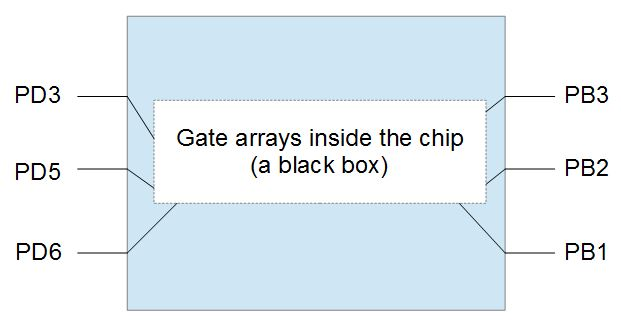
\includegraphics[width=0.6\linewidth]{picture/mcu}
\caption{Arduino MCU}
\label{fig:mcu}
\end{figure}
The micro controller platforms are similar to the FPGA ones, and in modern times, the MCU producers will release tools called MicroController Abstract for the programmers to \textit{translate} the high-level programming language, normally C, into the hardware languages that micro controllers can understand. Programmers know the architecture of the MCU their programs run on, and uses modern programming languages to manipulate the signals and clock triggers. Both the input and output of the MCU can be \textit{translated} by the MicroController Abstract layer into the high level programming format. Take the Arduino MCU platform for example: the MCU can produce six modulated electric pulses on its six pins showed in picture \ref{fig:mcu}.\\
An example code for setting and reading the a value from pin $PD3$ is:
\begin{lstlisting}[breaklines,breakatwhitespace,caption={Reading PD3 from Arduino MCU},label=compression-psudoCode]
void setup() {
	Serial.begin(9600);
}
void loop() {
	int sensorValue = analogRead(PD3);
	Serial.println(sensorValue);
	delay(1);
}
\end{lstlisting}
The MCU works in this way: in the setup phase, the program set serial frequency to be 9600 bit per second as the data frequency of the pins, then the MCU is read for sending and receiving signals for each available pin, and in this example we read the default value of pin $PD3$ by using the method analogRead(). This function in the hardware abstract layer will be translated to a pulse which goes into the circus, and gain the module of ping $PD3$ signal within a system circle, and goes back to the hardware abstract layer. They layer will again translate the signals into a high level programming format, for example, if the black box attaches the $PD3$ pin to a high voltage source of 5 Volt, the abstract layer will translate the module 5 Volt into an integer of one.\\
The expression of different signals can be fixed by the manufacture or defined by the programmers, however, the key idea is that the black box which controls the behaviours of pins must be known to the system designers, and everything inside the black box is fixed and unchangeable, especially the modular logics within.Therefore, the design process of the MCU platform programs are:
\begin{itemize}
	\item[1.] Choose and understand the hardware logics of the MCU board
	\item[2.] Design the software which uses the functions provided by the hardware
\end{itemize}
A good example are the MCU chips in the heat sensors, which receives the signals of sensors it attaches to and the outputs are distance from the source to sensor, and a pair of coordinates indicating the relative positions of source. Programmers can make use of the outputs to design their programs, varying from an intelligent flushing toilet controller to navigating program in heat guided missiles.\\ 
\subsubsection{The FPGA platform}
The FPGA and microcontroller platform is quite similar, as both needs to know the detailed hardware implementations, and a hardware abstract layer to translate the programming languages and runtime signals.\\
The difference between the two is FPGA platforms do not have a \textit{fixed} module logics showed in the picture \ref{fig:mcu}, and the designing process of FPGA platform has two phases:
\begin{itemize}
	\item[1.] Design the module logics
	\item[2.] Design the software which uses the module logics in the FPGA
\end{itemize}
This process looks complex in the first place, because the module logic in FPGA chip is designed by the programmer, so the software needs to contain a full implementation of hardware abstract layer to perform the bi-directional translation. Programming on FPGA was difficult in the early times, however, the modern design of FPGA boards absorbs the advantages in MCU and FPGA, and creates an structure illustrated in the following picture:
\begin{figure}[H]
\centering
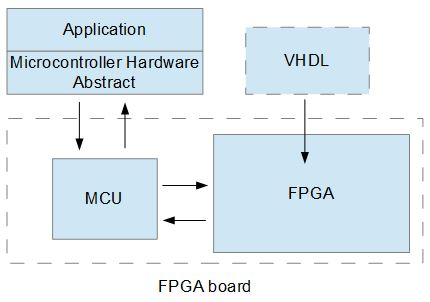
\includegraphics[width=0.5\linewidth]{picture/fpgadesign}
\caption{Modern FPGA design}
\label{fig:fpgadesign}
\end{figure}
The programmer nowadays do not need to worry about the hardware interfaces of FPGA chip, as the manufacturers have implemented an MCU over the FPGA, and setup the interfaces via MCU instead of the FPGA directly. As discussed above, the MCU has fixed interfaces, and the MCU on the FPGA board provides fixed general interfaces for applications to invoke, and fetch the data from FPGA. The advantage of using this middle ware structure is that the programmers do not need to care about the hardware implementation of the FPGA itself, and manufacturers can provide general drivers for the MCU over specific operating systems, with which the FPGA computation resources can be abstracted into an function in high level programming languages.\\
\subsubsection{Spartan-6 with Raspberry Pi2}
The Spartan-6 FPGA over Raspberry Pi, the Logi Pi follows similar way, and it does not use the MCU but rather a technology called Wishbone to create a seamless communication between the CPU and FPGA. It uses Spartan-6 FPGA chip the hardware interfaces to connect to the Raspberry Pi board, supporting Linux based system, and programs can be burnt into the FPGA directly via general tools.\\
The advantage of using Wishbone will be discussed later, and for introduction, the Wishbone abstracts the MCU discussed above for running programs in FPGA and communicate with CPU. It is an abstract layer which now support Python and C programming language.\\

\subsection{FPGA hardware programming}
As discussed above, the FPGA programming involves two aspects, the software part which communicates with the FPGA, and the FPGA module logic which simulates the function of a MCU. This section will discuss the latter part, and show how this project works with the FPGA hardware design.\\
Program the hardware logic module in FPGA forms the following steps:
\begin{itemize}
	\item Understand the board structure: input and output signals
	\item Design the hardware logic inside the FPGA chip
	\item Programming the logic into FPGA and test
\end{itemize}
\subsubsection{Board structure}
The first step is to understand the board design, including understand the hardware resources we have on the board. For example, we need an accumulator to perform a for-loop, however, we need to know which pin refers to the clock on board, to trigger every step of the loop. In the Logi Pi v1.5 board, the clock can be triggered by an oscillator with standard 50MHz signal source, and connects to the $P85$ pin. \\
Usually, the pins of the FPGA chip are bounded into banks, so the electric schema of FPGA chips will show the pin structure as a form of banks. The FPGA manufacturers do not know the components outside the chip itself, however, only the creator of FPGA board can know how the board structure looks like. The design of FPGA application functions needs a file describes it, to avoid checking schematics diagrams every time, including the number, name and function of each pin on the FPGA chip, therefore we can use the hardware description language(HDL) to implement our functions.\\
\subsubsection{Design the hardware logic}
The second step is to understand the function need to implement: how the signals are imported into the FPGA, and how the output is consumed. The signals are variables that are created in the applications running on the CPU platform, and we have the Wishbone mechanism to slurp the signals from the memory in CPU to the SDRAM on the FPGA board, and push them into the designed pin. \\
Design of the hardware logic in FPGA follows the idea of modular programming, and the designer needs to split the hardware design into basic modules according to the functions FPGA chip provided. Each module is consisted of three parts: the input, which can be a system signal like clock, or the output from another module; the basic logic which contains the hardware logic of how a signal is processed by the basic components, for example the pulse-width modulation logic to carry a constant signal with a periodic one using the following logic:
\begin{lstlisting}[breaklines,breakatwhitespace,caption={PWM module in Verilog},label=compression-psudoCode]
//module begin
input clk_in;
input [7:0] sig_in;
input [7:0] counter;

output reg PWM_out =0;
always@ (poseedge clk_in) 
	begin
		if(counter < sig_in)
			PWM_out <= 1;
		else
			PWM_out <=0;
		counter <= counter +1;
	end
//module end		
\end{lstlisting}  
The example code shows how to carry an eight-bit long constant signal with the provided system clock, and can be presented in the picture \ref{fig:pwm}. This diagram is the basic component of the hardware design, which we introduces to illustrate how the basic components discussed above are connected together as an overall hardware logic, to perform certain algorithm.\\
The benefit of using the modular design is that the modules are reusable, and the basic logic components inside FPGA is barely changed, so we can always reuse some classic solution even the code is decades ago.\\
The Logi Pi FPGA chip supports most of the modular design in the VHDL library, and the manufacturer developed some customized interfaces mainly for chip-to-chip communication especially for the ARM based platforms via PCI ports. These interfaces are the basic parts of this project, called Wishbone and will be discussed later.\\  
\begin{figure}[H]
\centering
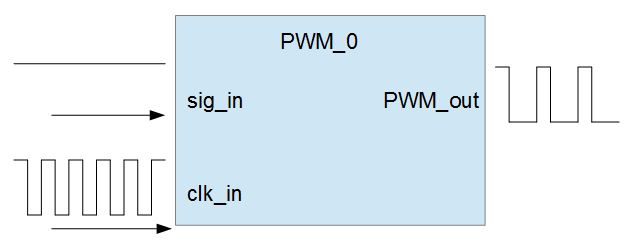
\includegraphics[width=0.5\linewidth]{picture/pwm}
\caption{PWM modular logic}
\label{fig:pwm}
\end{figure}
\subsubsection{Burning the design into the FPGA chip}
The FPGA chips are reprogrammable, and the programmer needs to make the chip aware the design using a hardware-based descriptive language to make the FPGA chips know how to form the proper hardware structures. There are several different hardware description languages, and them main stream are the Verilog and VHDL. This project will not introduce or compare these two HDLs, as both are well-known and widely implemented over both academic and commercial fields. Most of the Logi Pi modular interfaces are designed using VHDL, and the project needs to reuse some of them, we choose VHDL as our programming language.\\
The hardware description language abstracts the hardware details, to improve the universality of the designs. Therefore the module design of input/output signals need a mapping procedure to find the correct hardware resources they combine to. This mapping is based on the descriptive file of the board mentioned above.\\
Design of the hardware logics always include reusable modules, and it is less likely that designers need to focus on the implementation of a simple module like PWM modules, and a library of implementation details is required when burning the design into the actual FPGA chips.\\
We have already known the board structure including input/output signal environments and the FPGA chip functions, we need to combine these information together to make the FPGA work as we designed:
\begin{itemize}
	\item Write and test the VHDL described design off board
	\item Introduce the hardware description file with UCF extension to link the modules to hardware interfaces
	\item Introduce the library to complete the detail design
\end{itemize}
The process now can be performed by the integrated development environment provided by Xilinx ISE tools. However, as the Spartan-6 is an old product and the ISE design suite is no longer supported by the Xilinx, there will be some difficulty in compiling the code, and will be explained in the system implementation chapter.\\
\begin{figure}
\centering
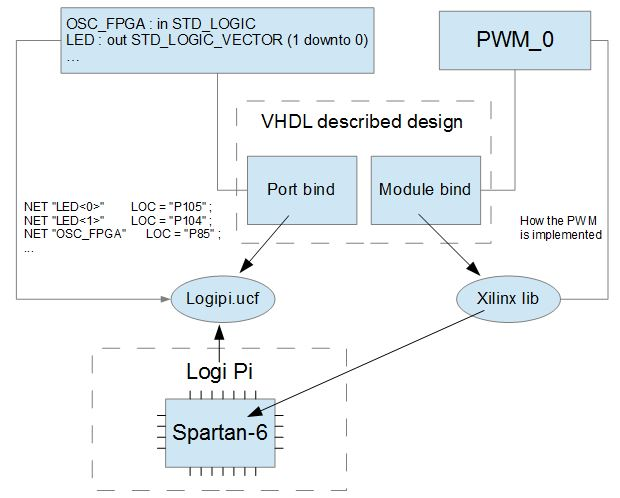
\includegraphics[width=0.7\linewidth]{picture/vhdlstruct}
\caption{VHDL file structure}
\label{fig:vhdlstruct}
\end{figure}
\subsection{Wishbone: interface for FPGA-to-PC communication}
We had a brief introduction in how the FPGA works in the above sections, however, the project requires communication between an CPU hosted application and a FPGA hosted one. An commonly used solution is the serial communication architecture, and the communication is via the universal asynchronous receiver/transmitter interfaces\cite{michael1992universal}. The architecture is in picture \ref{fig:uart}.However, the UART technology is an overkill in this project, as the Logi Pi FPGA board is connected to the Raspberry Pi via the GPIO ports, and we can use the serial peripheral interface bus to implement the communication instead.\\
\begin{figure}[H]
	\centering
	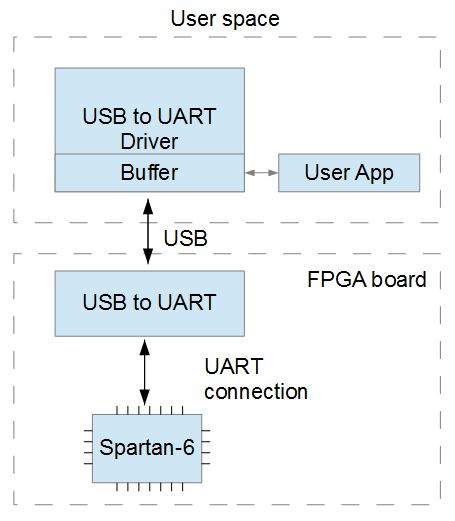
\includegraphics[width=0.5\linewidth]{picture/uart}
	\caption{UART architecture}
	\label{fig:uart}
\end{figure}
\subsubsection{Serial Peripheral Interface on Raspberry Pi}
SPI solves the problem of visibility of FPGA modular details on the application side. Without SPI, the applications need to know the exact hardware layers between the FPGA pins and the GPIO ports it connects to, and all the read/write performances need to call a chain of hardware data drivers to make the communication work. However, the SPI isolates the banks by tagging the FPGA pins with addresses, and ideally, the applications on CPU side only need to know the virtual address it connects to, and the SPI layer will deal with rest of the details.\\ 
The structure of SPI is quite simple, which is consisted of a master and a slave. The master is embedded on the Raspberry Pi board forming two pairs of communication channel, a slave select channel and a clock:
\begin{itemize}
	\item Master Output Slave Input: data is the output of the master SPI and the slave receives the data
	\item Master Input Slave Output: master SPI receives, or reads the data from slave, however, the slave normally cannot invoke this channel
	\item Slave Select: the master SPI can select different slaves if there were multiple implementation of slaves in the FPGA
	\item Serial Clock: the master can output an clock signal instead of the build-in clock signal on the board
\end{itemize}
The Raspberry Pi disables the SPI driver by default\cite{rasppispi}, however, it is easy to unlock it by using the tool \textit{RASPI-CONFIG} provided by Alex Bradbury to unblock it\cite{rasppiconfig}. The communication of SPI showed in schematic diagrams \ref{fig:spi}. The SPI slave port connects to both the Spartan 6 FPGA chip and the SDRAM chip on the Logi Pi board, and we can use the SDRAM to store big data.\\
\begin{figure}[H]
\centering
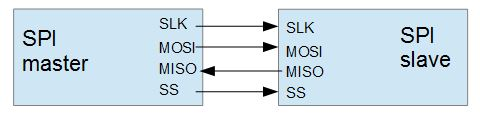
\includegraphics[width=0.5\linewidth]{picture/spi}
\caption{SPI schematic diagram}
\label{fig:spi}
\end{figure}
\subsubsection{Implementation of Wishbone on Logi Pi}
The SPI solve the problem of data driver using GPIO ports communication, however, the implementation over pure SPI is still too complicate to achieve. The application on the CPU side still needs to know the implementation details of the FPGA side, for example, the choice of SPI slaves is triggered by the application, however, different FPGA chip may have varieties of slave memory access address according to the compiling environment for the VHDL. Wishbone technology provides an alternative solution that wraps up the SPI interconnection details into high-level programming language libraries, and combined with address mapping tool provided, the applications on CPU side can have a relatively \textit{fixed} call addresses.\\
This design sacrifices some flexibility and achieve much convince as designers do not need to reimplement any communication interfaces any more.\\
The basic component of Wishbone is the register, which has a relatively \textit{fixed} address usually starts with $0x0$ with an offset $0x1$. It is the basic interface for all the wishbone logics and has 16-bit input/output\cite{logiwishbone}.\\
\begin{figure}[H]
\centering
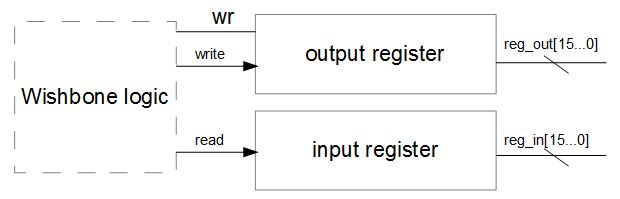
\includegraphics[width=0.6\linewidth]{picture/wishbone_register}
\caption{Wishbone register}
\label{fig:wishbone_register}
\end{figure}
As mentioned above, the input and output processes are abstracted by the Wishbone wrapper. Take Python for example, reading and writing with register $0x0$ can be performed using the two functions provided by the library \textit{logiRead} and \textit{logiWrite}:
\begin{table}[]
	\centering
	\caption{My caption}
	\label{my-label}
	\begin{tabular}{@{}lll@{}}
		\toprule
		Parameter                                                    & Function                                                     & Notes                                                                                                                                                                                       \\ \midrule
		address                                                      & \begin{tabular}[c]{@{}l@{}}logiWrite\\ logiRead\end{tabular} & the read/write destination address in hex format                                                                                                                                            \\
		\begin{tabular}[c]{@{}l@{}}high-byte\\ low-byte\end{tabular} & logiWrite                                                    & \begin{tabular}[c]{@{}l@{}}the write content in hex format and the string will\\  be converted to ASCII. It has a pair of parameters \\ because the registers are 2 bytes long\end{tabular} \\
		length                                                       & logiRead                                                     & define the byte it reads, 2 means read the entire 16 bits                                                                                                                                   \\ \bottomrule
	\end{tabular}
\end{table}
This project does not have any peripherals and the hardware algorithms are implemented via the basic input/output processes. So the application on the MPI side needs to communicate with the registers via Wishbone, and the algorithms are performed after the data is sent to the registers. After receiving the data from Wishbone bus, we can implement the hardware algorithms afterwards.\\
\subsubsection{Parallel process and FPGA status}
The FPGA processes are running parallel with the applications on CPU side, and the application design should take this into consideration. The processing speed of FPGA is much faster than the normal CPU hosted applications, and the clock frequency is different between the cluster. The Wishbone mechanism synchronise the clock via transmission layer, however, the application inside the FPGA still needs to wait for the read signal from the application.\\
Another problem is that the status of FPGA is controlled by the electric signals only, and the interfaces are fixed. Therefore if the application on the CPU does not read from the FPGA first and change the status of FPGA, the processing result in FPGA modular will soon lost before the CPU applications can react.\\
These two features requires the design of the system to be aware of the execution sequences especially in the FPGA communication.\\
\subsection{Conclusion}
This section introduces how the FPGA will work with the receiver applications on the MPI-CH structure, and focuses on how to design and implement a hardware algorithm in the FPGA, from design to actual coding, and the important technology which enables the hardware to seamlessly communicate to the CPU hosted applications using Wishbone. The FPGA accelerated computation is widely used in the commercial solution to similar problems, especially in the market data feed handlers, however, this project shows the potential of using an open-source FPGA board to achieve the same goal over an cluster hardware environment.\\ 
\chapter{Experiment Design, Requirements and Expectations}
This chapter shows the design of experiment, requirements and expectations the project wants to achieve. \\
The main goal is to implement a data processor for the dual feed data sources using open-source hardware, and implement UDP package processing application on the FPGA for acceleration.\\
In order to achieve the goal of receiving dual feeds, which will come from physically two Ethernet cables, the system needs at least two Ethernet ports, and we introduces MPICH over multiple independent hardware which has one Ethernet port each, and congregate them into a cluster in order to meet the requirements.\\
\newpage
\section{Experiment Design}
This section introduces the design of five experiments and their architectures:
% Please add the following required packages to your document preamble:
% \usepackage{booktabs}
\begin{table}[H]
	\centering
	\caption{Experiment design table}
	\label{my-label}
	\begin{tabular}{@{}lll@{}}
		\toprule
		Number & Name                                                                                                   & Introduction                                                                                                                                                                  \\ \midrule
		1      & Single data feedwith single receiver                                                                   & Normal UDP send/receive pair                                                                                                                                                  \\
		2      & Dual data feeds over the cluster                                                                       & \begin{tabular}[c]{@{}l@{}}Using dual data feeds of normal \\ UDP send/receiver pairs\end{tabular}                                                                            \\
		3      & \begin{tabular}[c]{@{}l@{}}Dual feeds processed with MPI \\ processors without RDMA\end{tabular}       & \begin{tabular}[c]{@{}l@{}}Using dual data feeds sending data\\ to MPI structure receivers without RDMA\end{tabular}                                                          \\
		4      & \begin{tabular}[c]{@{}l@{}}Dual feeds processed with MPI \\ processors with RDMA\end{tabular}          & \begin{tabular}[c]{@{}l@{}}Using dual data feeds sending data\\ to MPI structure receivers with RDMA\end{tabular}                                                             \\
		5      & \begin{tabular}[c]{@{}l@{}}Dual feeds processed with MPI \\ with unified QoS check\end{tabular}        & \begin{tabular}[c]{@{}l@{}}Ignoring the QoS check of sockets when\\ each node receives data, and performs an\\ unified checksum after merging the feeds\end{tabular}          \\
		6      & \begin{tabular}[c]{@{}l@{}}Dual feeds processed with MPI\\ with unified QoS check on FPGA\end{tabular} & \begin{tabular}[c]{@{}l@{}}Ignoring the QoS check of sockets when\\ each node receives data and performs an\\ unified checksum after merging the feeds\\ by FPGA\end{tabular} \\ \bottomrule
	\end{tabular}
\end{table}
\subsection{Experiment 1: Single data feed with single receiver}
This experiment shows the behaviour of a single UDP sender(data source) and a single UDP receiver(client), and tracks the output of receiver in the following environment:
\begin{itemize}
	\item No data lost in source and transmission
	\item Data lost in source
	\item Significant latency in data transmission
	\item Data source goes down
\end{itemize} 
This experiment requires an computer simulating the data source, and a raspberry pi hosted receiver as the client. Quality of service strategy of data transmission is relied on the default settings of the client operating system.\\
\begin{figure}[H]
\centering
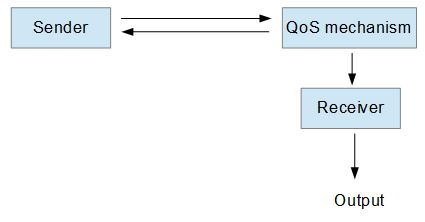
\includegraphics[width=0.5\linewidth]{picture/Exp1}
\caption{Design of experiment 1}
\label{fig:Exp1}
\end{figure}
\subsection{Experiment 2: Dual data feeds over the cluster}
This experiment shows the advantage of using dual feeds. Data source needs to simulate two data sources with the same content in package, and has an manual offset of one millisecond. The experiment needs to track the output from receivers under the following scenarios:
\begin{itemize}
	\item No data lost in either sources
	\item One of the source simulates data lost, while the other does not
	\item Both sources have data lost
	\item One of the sources goes off-line, while the other one does not
	\item Both sources go off-line
\end{itemize}
The design is shown in picture \ref{fig:Exp2}.\\
Receiver 1 and 2 can communicate with each other using network protocols and contact $output_{1}$ and $output_{2}$ together to have an unified output, and shows the differences in data lost conditions.\\
The QoS mechanism is also relied on the configurations in operating system of the receiver, and the merging process will happen in the simulated master node.\\ 
\subsection{Experiment 3: Dual feeds processed with MPI processors without RDMA}
This experiment implements MPICH over the Raspberry Pi2 clusters, and the experiment shows output on the master node with dual data feed sources under the same scenarios as experiment2. The receiver programme communicate with each other using the message passing interfaces provided by MPICH, and shows the details of latency handling.\\
The MPICH program uses MPI\_recv and MPI\_send pair to communicate under the MPI framework, and the way it runs is using SSH client in the master to perform \textit{mpiexec} shell command, with the arguments of a file containing lists of servers, and configurations of pointing at the destination of each MPI programme.\\
\begin{figure}[H]
\centering
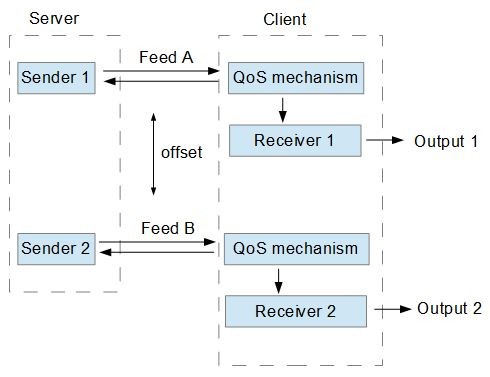
\includegraphics[width=0.7\linewidth]{picture/Exp2}
\caption{Design of experiment 2}
\label{fig:Exp2}
\end{figure}

\begin{figure}[H]
\centering
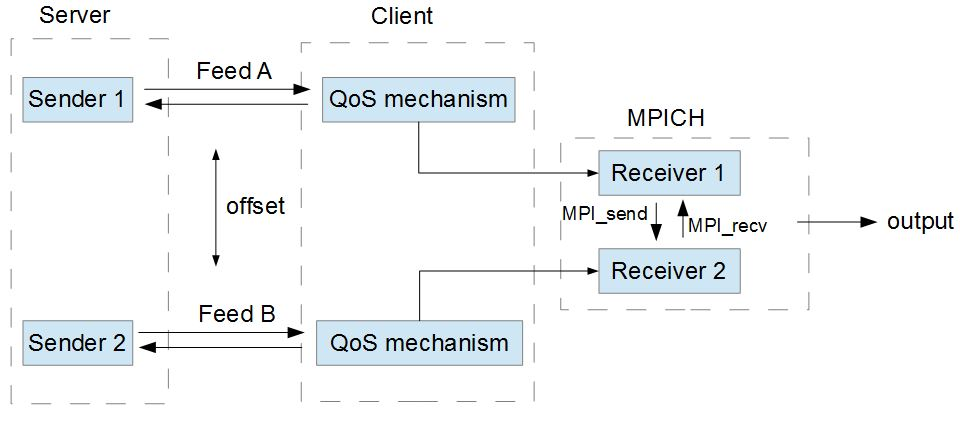
\includegraphics[width=0.8\linewidth]{picture/exp3}
\caption{Design of experiment 3}
\label{fig:exp3}
\end{figure}

\subsubsection{Description}
This experiment shows the 
\begin{itemize}
	\item UDP clients runs independently on two nodes, and passing the result to a master node
	\item UDP clients
\end{itemize}

\section{Experiment Requirements and Expectations}
\subsection{Simulation of the data source}
An server needs to run on an separate computer to simulate two high-frequency data sources, and push the data via different programming interfaces to two destinations.
\chapter{System Design and Implementation}
This part of the thesis explains design of the system, and the implementations of technologies discussed above. This part is consisted of three parts:
% Please add the following required packages to your document preamble:
% \usepackage{booktabs}
\begin{table}[H]
	\centering
	\caption{Contents of system design and implementation}
	\label{my-label}
	\begin{tabular}{@{}ll@{}}
		\toprule
		Title            & Content                                                                                                                                                                    \\ \midrule
		Hardware design  & \begin{tabular}[c]{@{}l@{}}The design of the hardware cluster, including the\\  actual hardware used, and the cabling strategy to \\ implement the dual feed.\end{tabular} \\ \hline
		Logical design   & \begin{tabular}[c]{@{}l@{}}Showing the logical interconnection of the cluster, \\ and the implementation of RDMA, MPICH and FPGA\end{tabular}                              \\ \hline
		Algorithm design & Showing the design of the algorithm processing dual feeds.                                                                                                                 \\ \bottomrule
	\end{tabular}
\end{table}
\newpage
\section{Hardware design}
The table of materials used in the project is shown in table \ref{bom}. However, we do not have 
\begin{table}[H]
	\centering
	\caption{Materials used in the experiment}
	\label{bom}
	\begin{tabular}{@{}llll@{}}
		\toprule
		Name                  & Amount & Manufacture    & Metrics                                                                                                                    \\ \midrule
		Raspberry Pi2         & 3      & Raspberry Org. & \begin{tabular}[c]{@{}l@{}}1x Boardcom ARM CPU, \\ 1x Ethernet Port, \\ 1x SD card port\\ 5.1V 1A input power\end{tabular} \\
		Kingston MicroSD card & 3      & Kingston       & 8GB Micro SD card                                                                                                          \\
		Logi Pi FPGA board    & 1      & ValentFX       & \begin{tabular}[c]{@{}l@{}}1x SPARTAN-6 FPGA chip, \\ 5V 1A input\end{tabular}                                             \\
		Ethernet hub          & 1      &                & \begin{tabular}[c]{@{}l@{}}1x S1786 central chip, \\ 8x Ethernet ports\end{tabular}                                        \\
		Ethernet cable        & 4      &                & RJ45 copper cable                                                                                                          \\
		Power source          & 1      & iClever        & \begin{tabular}[c]{@{}l@{}}6x Powerports, \\ 100-240V 50-60Hz 1200mA input, \\ 5V(max) each output\end{tabular}            \\
		Power cable           & 4      &                & USB power cable                                                                                                            \\ \bottomrule
	\end{tabular}
\end{table}
\section{Logical design}
The logic design of the project can be illustrated as the picture below:
\begin{figure}[H]
	\centering
	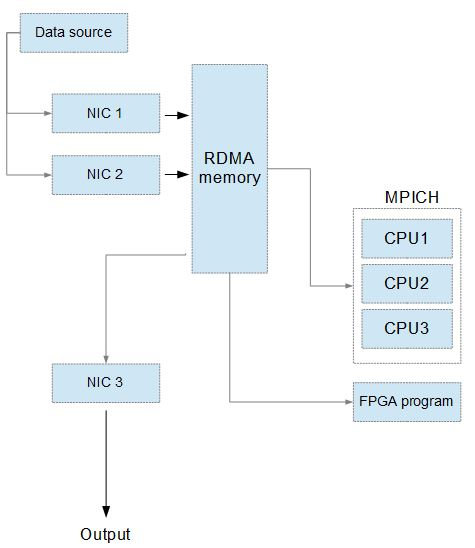
\includegraphics[width=0.5\linewidth]{picture/LogicDesign}
	\caption{The logic design of the system}
	\label{fig:LogicDesign}
\end{figure}
\section{Algorithm design}
\dots design of the thread dispatching, event sensor in the master board
\chapter{Implementation and Testing}
This is the chapter in which you review the implementation and testing
decisions and issues, and critique these processes.

Code can be output inline using \verb@\lstinline|some code|@.  For example,
this code is inline: \lstinline|public static int example = 0;|  (I have
used the character \verb@|@ as a delimiter, but any non-reserved character
not in the code text can be used.)

Code snippets can be output using the \verb|\begin{lstlisting} ... \end{lstlisting}|
environment with the code given in the environment.  For
example, consider listing \ref{Example-Code}, below.

\begin{lstlisting}[breaklines,breakatwhitespace,caption={Example code},label=Example-Code]
public static void main() {

  System.out.println("Hello World");

}
\end{lstlisting}

Code listings are produced using the package ``Listings''.  This has many
useful options, so have a look at the package documentation for further
ideas.


\chapter{Results}
This is the chapter in which you review the outcomes, and
critique the outcomes process.  You may include user evaluation here
too.


%%
%% Now we are back to the standard project contents that you should include
%%

\chapter{Conclusions}
%% Uncomment this to include a separate tex file wih the conclusion contents
%\include{conclusion.tex}

This is the chapter in which you review the major achievements in the
light of your original objectives, critique the process, critique your
own learning and identify possible future work.


\bibliography{ExampleBibFile}


\appendix

%%
%% Use the appendix for major chunks of detailed work, such as these. Tailor
%% these to your own requirements
%%

\chapter{Design Diagrams}

\chapter{User Documentation}

\chapter{Raw results output}

\chapter{Code}

%%
%% NOTE that for this to typeset correctly, ensure you use the pdflatex
%%      command in preference to the latex command.  If you do not have
%%      the pdflatex command, you will need to remove the landscape and
%%      multicols tags and just make do with single column listing output
%%

\begin{landscape}
\begin{multicols}{2}
\section{File: yourCodeFile.java}
\lstinputlisting[basicstyle=\scriptsize]{yourCodeFile.java}
\end{multicols}
\end{landscape}

\end{document}

%%% Local Variables:
%%% mode: latex
%%% TeX-master: t
%%% End:
